\chapter{Implementacja środowiska badawczego}
W niniejszym rozdziale przedstawiono proces implementacji środowiska badawczego pod kątem realizacji zdefiniowanych uprzednio scenariuszy badawczych. Spośród składowych omawianego procesu wyróznić należy: przygotowanie odmian topologii fizycznych środowiska w zależności od scenariusza badawczego, budowę interfejsów programowania aplikacji z wykorzystaniem porównywanych technologii, czy też zastosowanie mechanizmów pozwalających na weryfikację działania API w aspekcie programowania współbieżnego. Ponadto, zaprezentowana została konfiguracja dedykowanych porównywanym technologiom platform chmurowych, a także struktura elementów składających się na plan testowy, identyfikujący przeprowadzoną ewaluację w ramach narzędzia przeznaczonego do realizacji badań.    
\section{Realizacja topologii fizycznych}
W zależności od scenariusza badawczego, wykorzystywanego w kontekście przeprowadzonych ewaluacji, zbudowanych zostało pięć odmiennych wariantów topologii fizycznych. Cztery spośród nich, tyczą się badań wykonywanych w środowisku lokalnym, natomiast piąta z topologii, związana jest z obserwacją funkcjonowania interfejsów programowania aplikacji uruchomionych w obrębie określonych platform chmurowych.

W odniesieniu do każdej z topologii zbudowanej w środowisku lokalnym, zauważyć należy fakt zastosowania techniki rozproszonego testowania \textit{(ang. Distributed Testing)}, a także jasny podział odpowiedzialności w kontekście wszystkich wykorzystywanych urządzeń. Procedura zbierania obserwacji za każdym razem realizowana jest wewnątrz odpowiednio dostosowanej lokalnej sieci komputerowej cechującej się brakiem dostępu do sieci Internet. Ponadto, w obszarze połączonych ze sobą urządzeń systemu komputerowego, dezaktywowane zostały protokoły i usługi sieciowe generujące cykliczne komunikaty rozgłoszeniowe. Dzięki temu, wyeliminowano błędy pomiarowe o charakterze niedeterministycznym.

Odwołując się do topologii sieciowej zbudowanej w środowisku rozległym, zauważyć należy odmienny sposób pozyskiwania informacji o czasie przetwarzania pojedynczego żądania. W tym przypadku, wykorzystywane narzędzie pomiarowe służy jako generator żądań, jednakże czasy odpowiedzi na żądanie, zwrócone przez to narzędzie nie mogą być brane pod uwagę. Informacja o czasie przetwarzania żądania zostaje dostarczana bezpośrednio z interfejsu programowania aplikacji.

\subsection*{Konfiguracja pierwsza lokalnej topologii fizycznej środowiska badawczego}
\label{sec:lokalne-srodowisko-badawcze-ver-1}
Pierwsza spośród lokalnych topologii fizycznych środowiska badawczego zastosowana została w celu badania wpływu wykorzystania odmiennych systemów bazodanowych na wydajność interfejsów programowania aplikacji.

W ramach niniejszej topologii, wyróżnić należy dwa interfejsy programowania aplikacji (tj. utworzone z wykorzystaniem technologii C\#/.NET oraz NodeJS/Express), komunikujące się z jednym z pięciu serwerów bazodanowych (tj. MySQL Server, PostgreSQL Server, Microsoft SQL Server, SQLite oraz MongoDB). W określonym momencie czasu, utrzymywane jest tylko jedno aktywne połączenie pomiędzy jednym z API a jednym z serwerów bazodanowych. Ponadto, wewnątrz lokalnej sieci komputerowej, wyróżnić należy urządzenie komunikacyjne którym jest router, a także trzy urządzenia końcowe. Pierwszy z hostów pełni rolę "dyrygenta testu", który dostarcza informacje o konfiguracji testowej bezpośrednio do dwóch pozostałych urządzeń końcowych. Te urządzenia z kolei, odpowiedzialne są za generowanie żądań zgodnie ze zdefiniowanym natężeniem, częstotliwością, a także czasem trwania ewaluacji. Każde z oddzielnych urządzeń fizycznych połączone jest z urządzeniem komunikacyjnym poprzez łącze przewodowe, o tej samej przepustowości (tj. 1Gb/s), a także identycznej kategorii przewodu (tj. kategoria 6).

Na ilustracji \ref{fig:topologia-1} przedstawiono schemat pierwszego wariantu lokalnej topologii fizycznej środowiska badawczego.

\begin{figure}[ht]
    \centering
     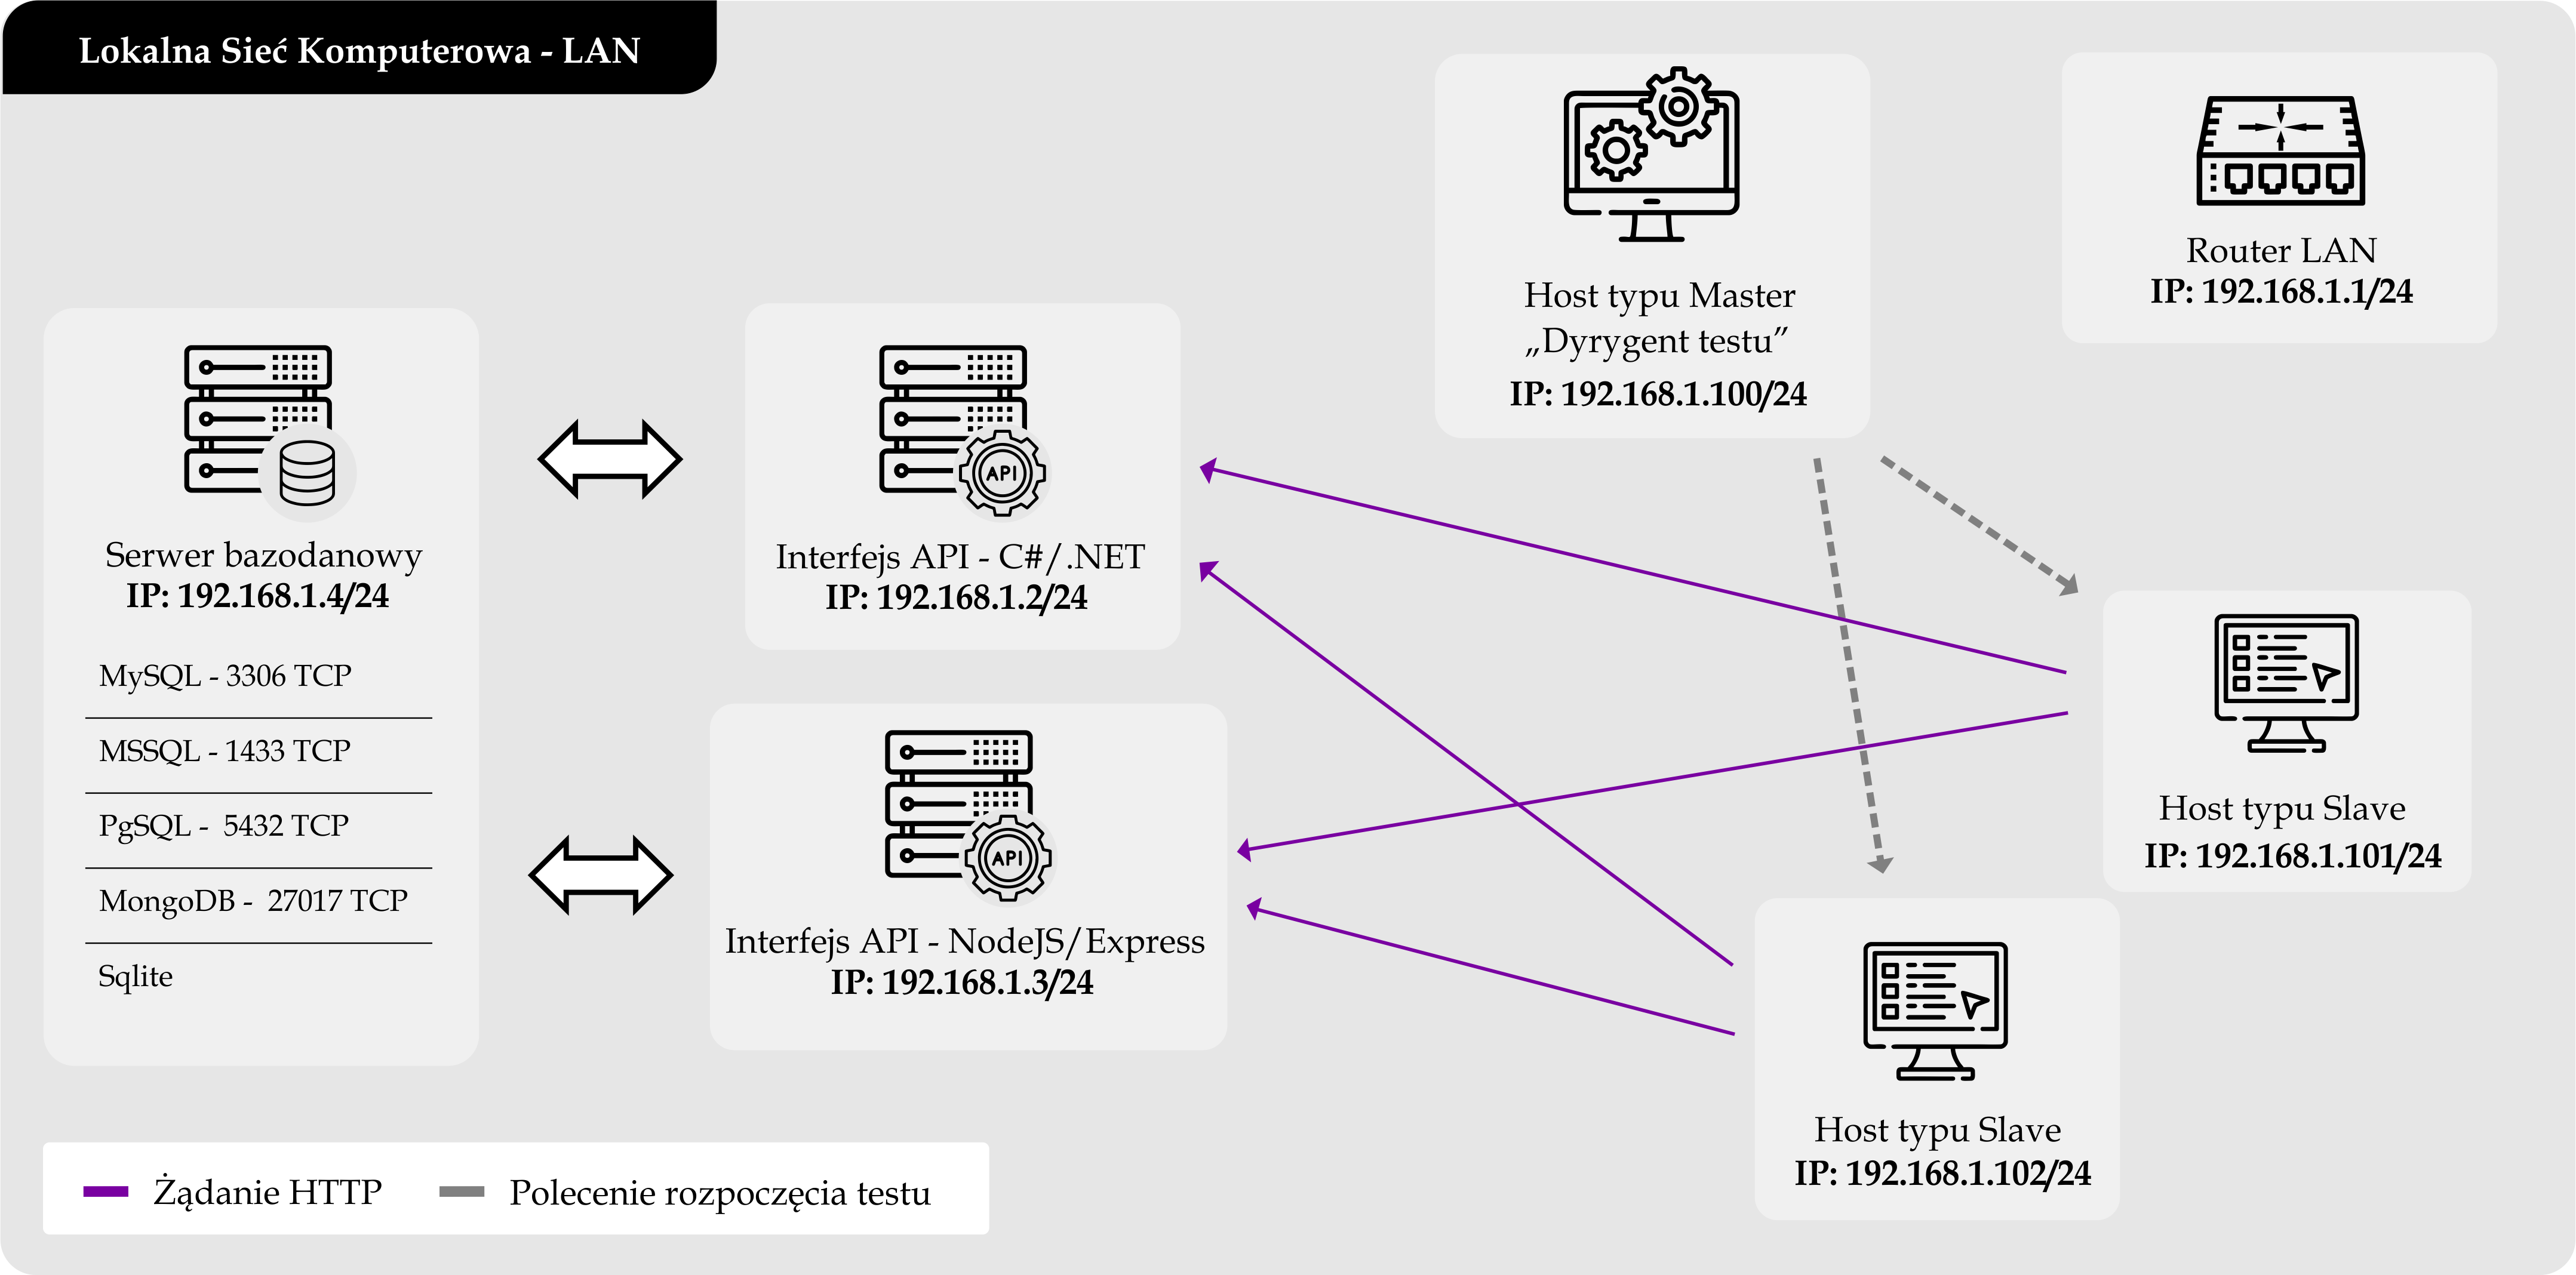
\includegraphics[width=\linewidth]{rys04/topologia-1.png}
    \caption{Konfiguracja pierwsza lokalnej topologii fizycznej środowiska badawczego}
    \label{fig:topologia-1}
\end{figure}

\subsection*{Konfiguracja druga lokalnej topologii fizycznej środowiska badawczego}
\label{sec:lokalne-srodowisko-badawcze-ver-2}
Druga topologia fizyczna środowiska badawczego, dotycząca ewaluacji w obrębie lokalnej sieci komputerowej, zbudowana została na potrzeby badań zaimplementowanych mechanizmów programowania współbieżnego, a także przechowywania odpowiedzi na żądania w ramach pamięci podręcznej.

W omawianej topologii wskazać należy dwa interfejsy programowania aplikacji, których implementacja dokonana została w porównywanych dwóch technologiach programistycznych. Obie usługi sieciowe, komunikują się z pojedyną instancją serwera bazodanowego - w przypadku badania pamięci cache, bądź też nie odwołują się do niego wcale - w przypadku badania efektywności operacji współbieżnych. Spośród urządzeń komunikacyjnych, wykorzystywanych do przeprowadzenia ewaluacji, wyróżnić należy jedno urządzenie typu Master (tzw. Dyrygent testu), a także jednego hosta typu Slave (tzw. generator żądań). Pierwszy z komputerów ma za zadanie przechowywać konfigurację wykonywanego badania, a także dostarczać komendy związane z rozpoczęciem i charakterystyką testu. Drugi host pełni rolę maszyny wytwarzającej i wysyłającej żądania protokołu hipertekstowego, zgodnie z koncepcją nakreśloną przez uzyskany plan ewaluacji. Wszystkie urządzenia znajdują się w obszarze pojedynczej, przewodowej lokalnej sieci komputerowej. Analogicznie do konfiguracji pierwszej, każde łącze przewodowe charakteryzuje się tym samym standardem oraz przepustowością.

Na ilustracji \ref{fig:topologia-2} przedstawiono schemat drugiego wariantu lokalnej topologii fizycznej środowiska badawczego.

\begin{figure}[ht]
    \centering
     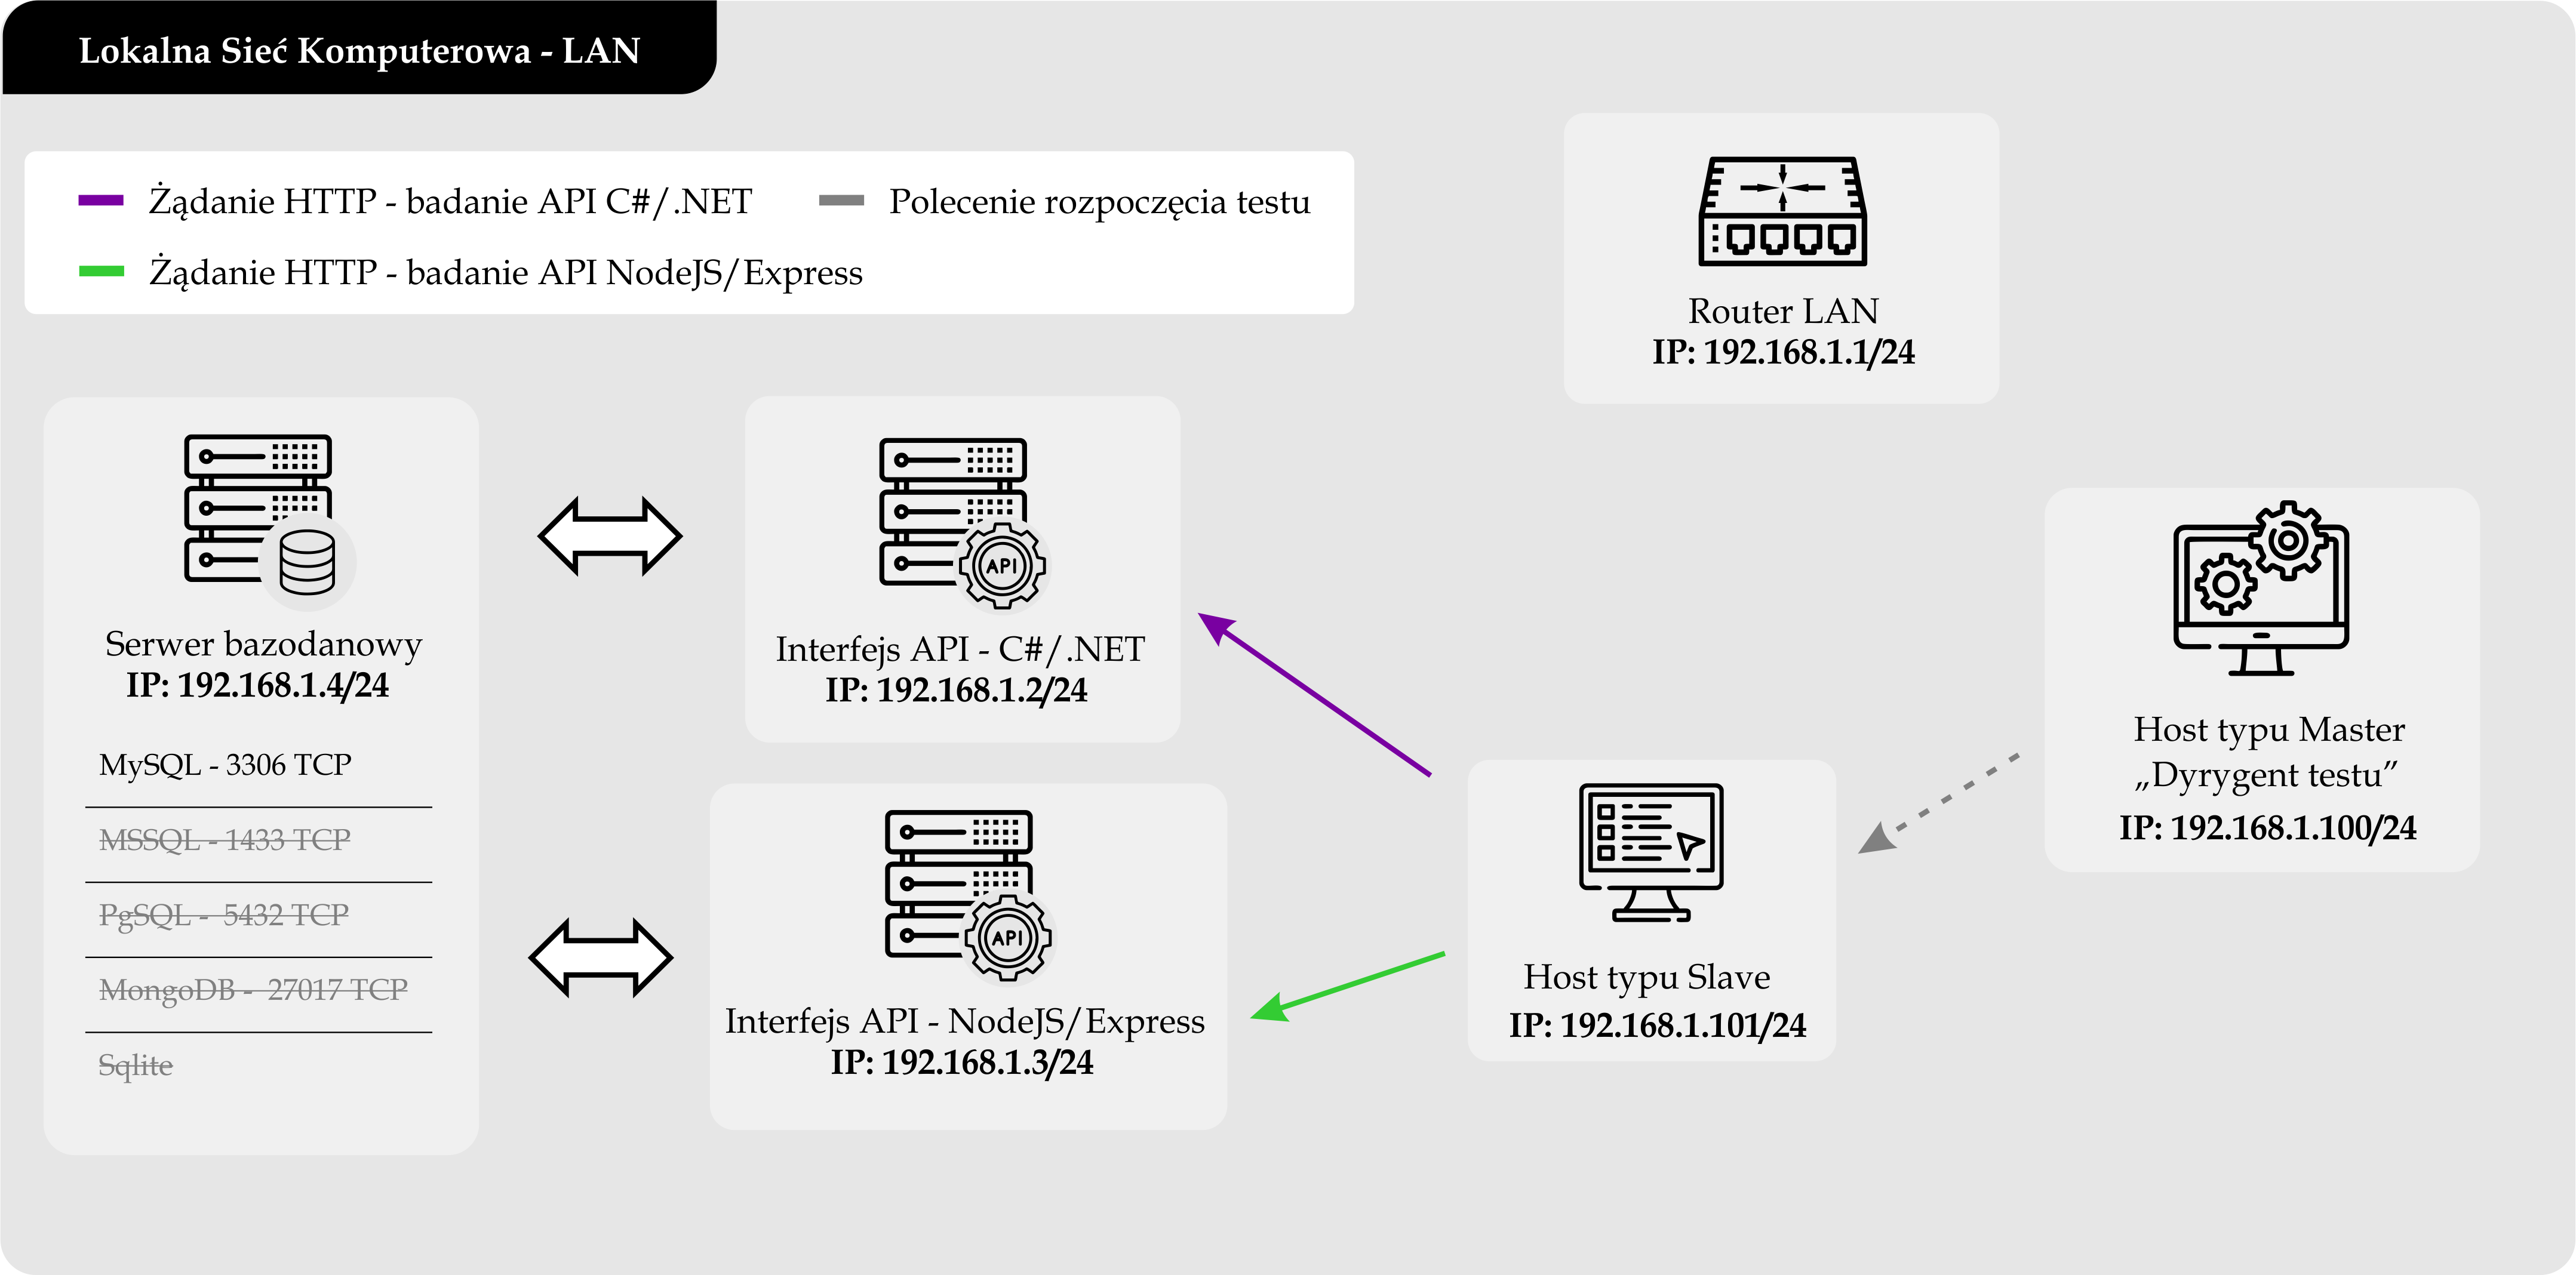
\includegraphics[width=\linewidth]{rys04/topologia-2.png}
    \caption{Konfiguracja druga lokalnej topologii fizycznej środowiska badawczego}
    \label{fig:topologia-2}
\end{figure}

\subsection*{Konfiguracja trzecia lokalnej topologii fizycznej środowiska badawczego}
\label{sec:lokalne-srodowisko-badawcze-ver-3}
Trzecia lokalna topologia fizyczna środowiska badawczego przystosowana została w celu umożliwienia realizacji badań dotyczących wydajności obsługi operacji asynchronicznych.

W schemacie tym, zauważyć można wystąpienie trzech interfejsów programowania aplikacji. Analogicznie do topologii opisanych powyżej, dwa spośród trzech API zaimplementowane są w technologiach będących przedmiotem analizy tej pracy. Trzecia usługa sieciowa, służy do udostępniania zgromadzonych w niej danych, w związku z czym posiada ona tylko i wyłącznie punkty końcowe obsługiwane z wykorzystaniem metody GET. Punkty styku ostatniego z interfejsów dostarczają funkcjonalności pobierania danych o zróżnicowanym rozmiarze.

Ponadto, zbieżnie do konfiguracji pierwszej lokalnego środowiska badawczego, wyszczególnić możemy dwa urządzenia końcowe w roli generatorów żądań, oraz jednego hosta działającego w trybie "Dyrygenta testu". Należy podkreślić, że ewaluacje dotyczące każdej z technologii, zarówno w scenariuszach badawczych wykorzystujących tę, jaki i pozostałe topologie, wykonywane są w odrębnych chwilach czasu. Implikuje to fakt, że połączenie pomiędzy hostem badającym, interfejsem badanym, a także interfejsem pomocniczym jest aktywne tylko dla aktualnie badanego rozwiązania technologicznego.

Poza interfejsami programowania aplikacji oraz urządzeniami końcowymi wskażać należy urządzenie sieciowe, jakim jest przewodowy router LAN, który łączy wszystkie elementy topologii w ramach pojedynczej sieci LAN. Standard oraz przepustowość wykorzystywanych łączy pozostaje niezmienna względem pierwszej oraz drugiej z topologii fizycznych.

Na ilustracji \ref{fig:topologia-3} przedstawiono schemat trzeciego wariantu lokalnej topologii fizycznej środowiska badawczego.

\begin{figure}[ht]
    \centering
     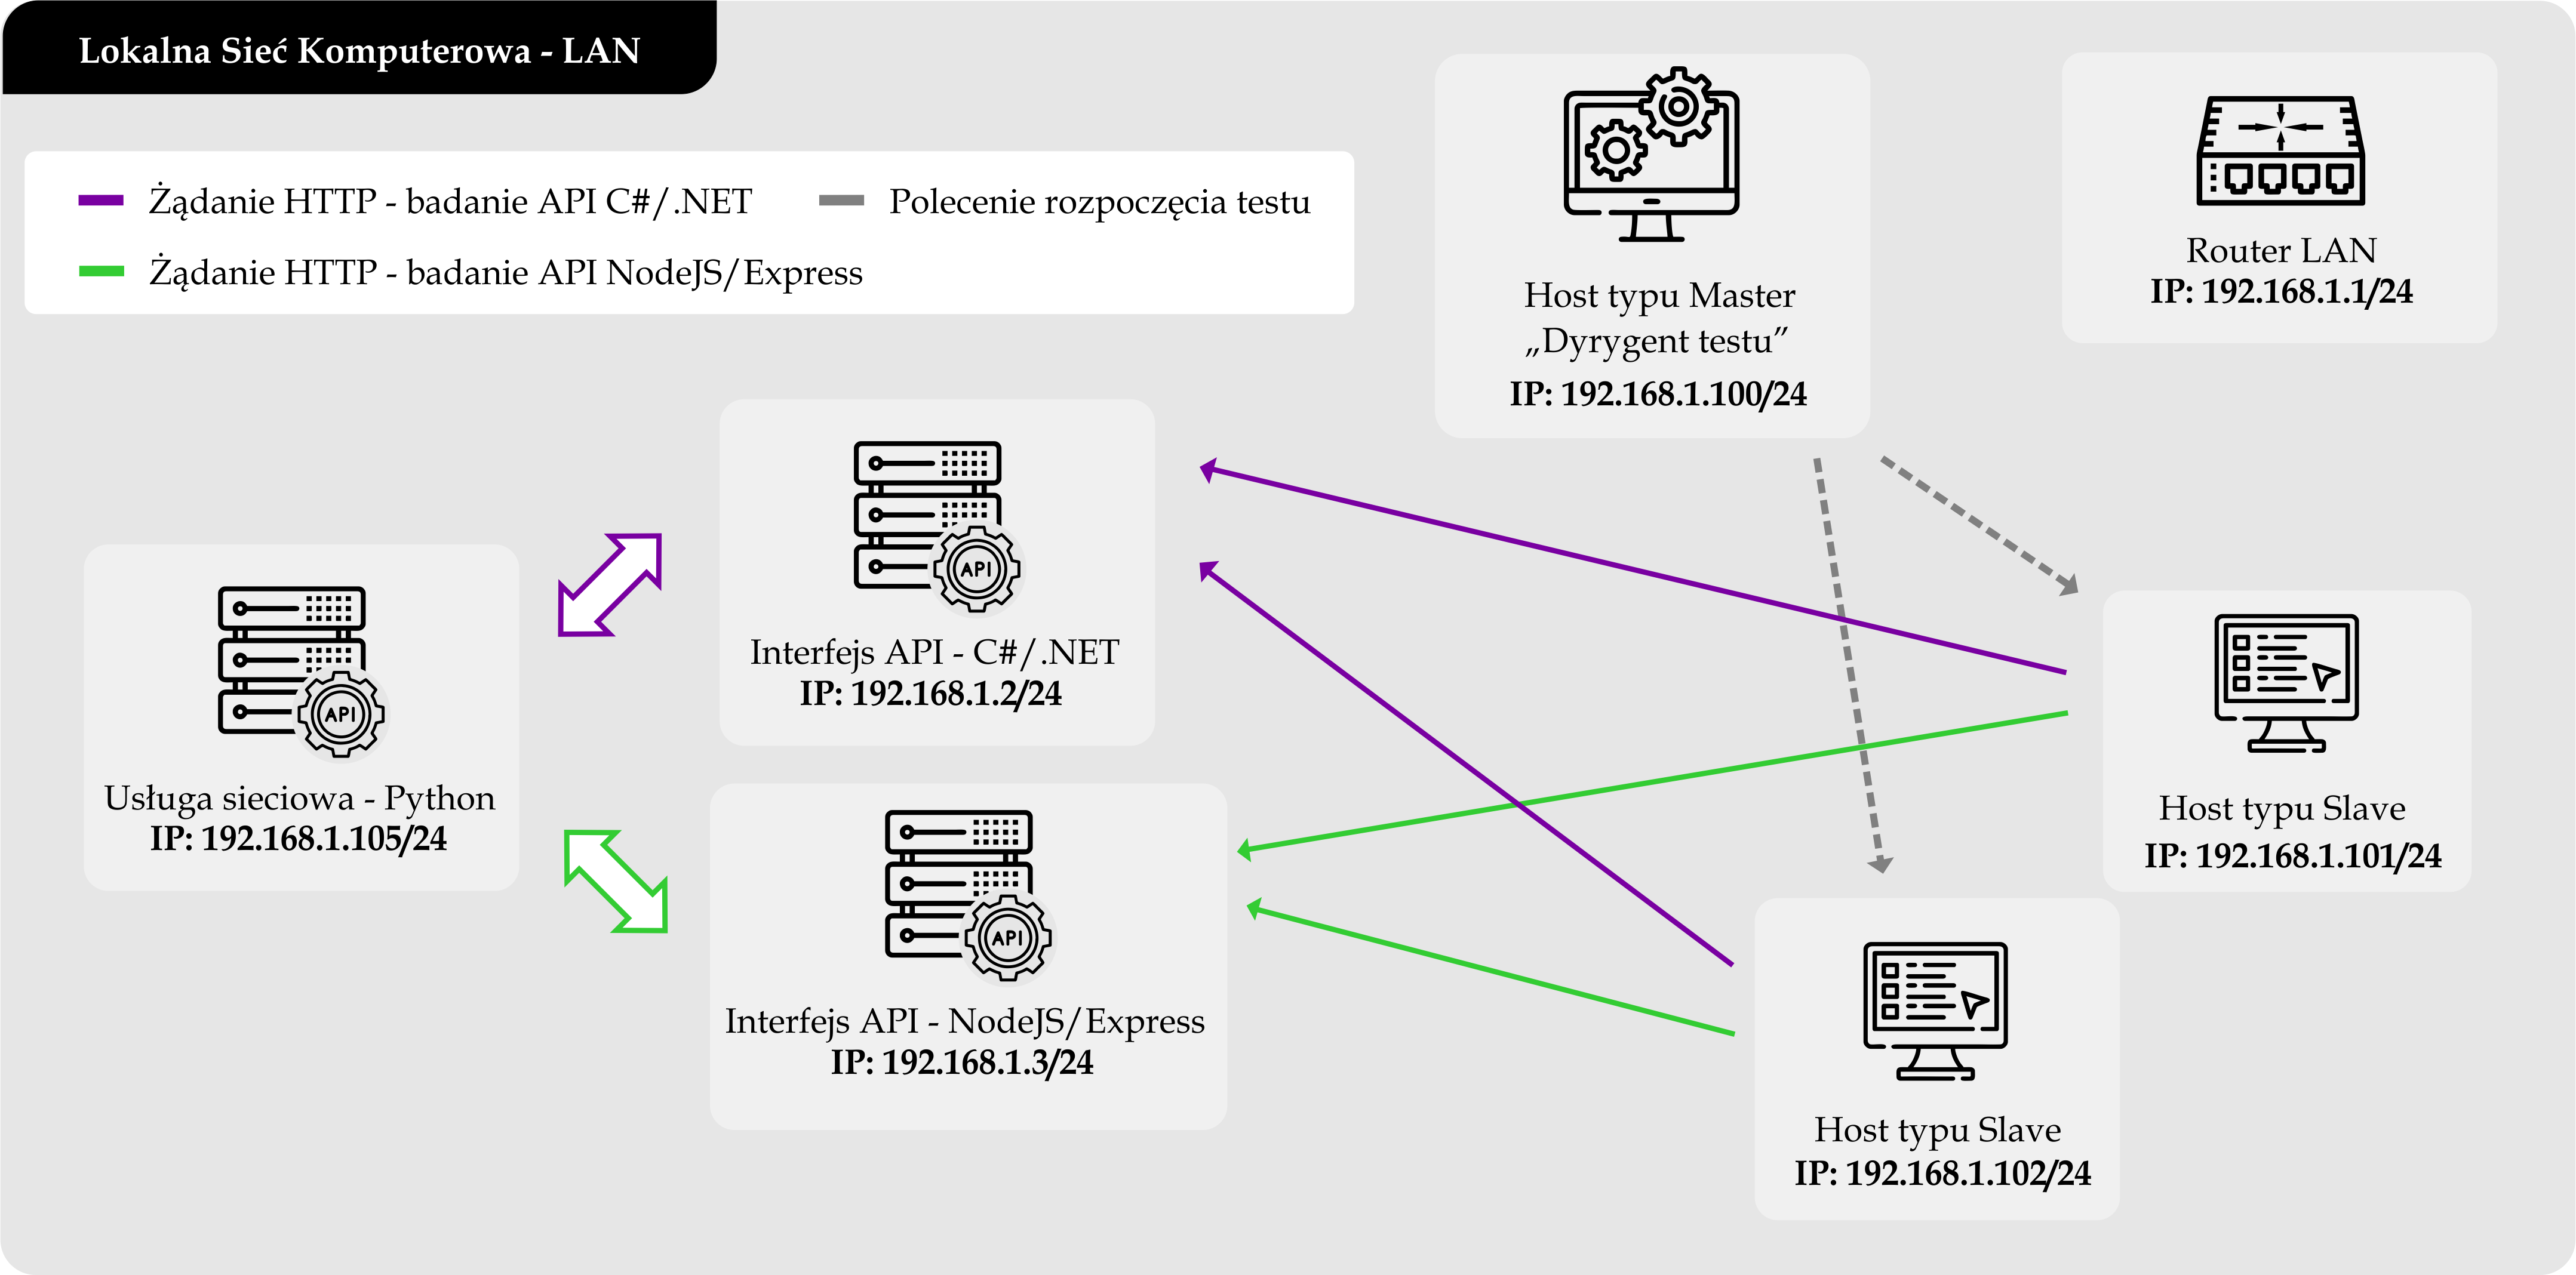
\includegraphics[width=\linewidth]{rys04/topologia-3.png}
    \caption{Konfiguracja trzecia lokalnej topologii fizycznej środowiska badawczego}
    \label{fig:topologia-3}
\end{figure}

\subsection*{Konfiguracja czwarta lokalnej topologii fizycznej środowiska badawczego}
\label{sec:lokalne-srodowisko-badawcze-ver-4}
Ostatnia z lokalnych topologii fizycznych środowiska badawczego zbudowana została w kontekście przeprowadzenia badania efektywności interfejsów programowania aplikacji w związku z zastosowaniem wzorca podziału odpowiedzialności.

Wykorzystanie tego wzorca, umożliwia separację zarówno modeli danych, jak i również fizycznych struktur bazodanowych. Dlatego też, w ramach omawianej topologii zdecydowano się na wprowadzenie dwóch oddzielnych serwerów baz danych. Serwer bazy danych wykorzystywany do zapisu implementuje operację replikacji transakcyjnej dzięki czemu, po wykonaniu zapisu do jednego źródła danych, zapisane informacje są automatycznie przenoszone do drugiej z baz. W ramach połączenia z serwerem bazodanowym wykorzystywanym do odczytu, po stronie interfejsów programowania aplikacji dokonano przystosowania modelu danych.

Poza serwerami danych, w ramach topologii wyróżnić należy dwa porównywane interfejsy programowania aplikacji, a także zbiór trzech urządzeń końcowych. Dwa spośród nich pełnią rolę generatorów żądań, natomiast trzeci host pracuje w trybie "dyrygenta testu". Wszystkie z urządzeń połączone są w obrębie lokalnej sieci komputerowej do urządzenia sieciowego którym jest router LAN.

Na ilustracji \ref{fig:topologia-5} przedstawiono schemat czwartego wariantu lokalnej topologii fizycznej środowiska badawczego.

\begin{figure}[ht]
    \centering
     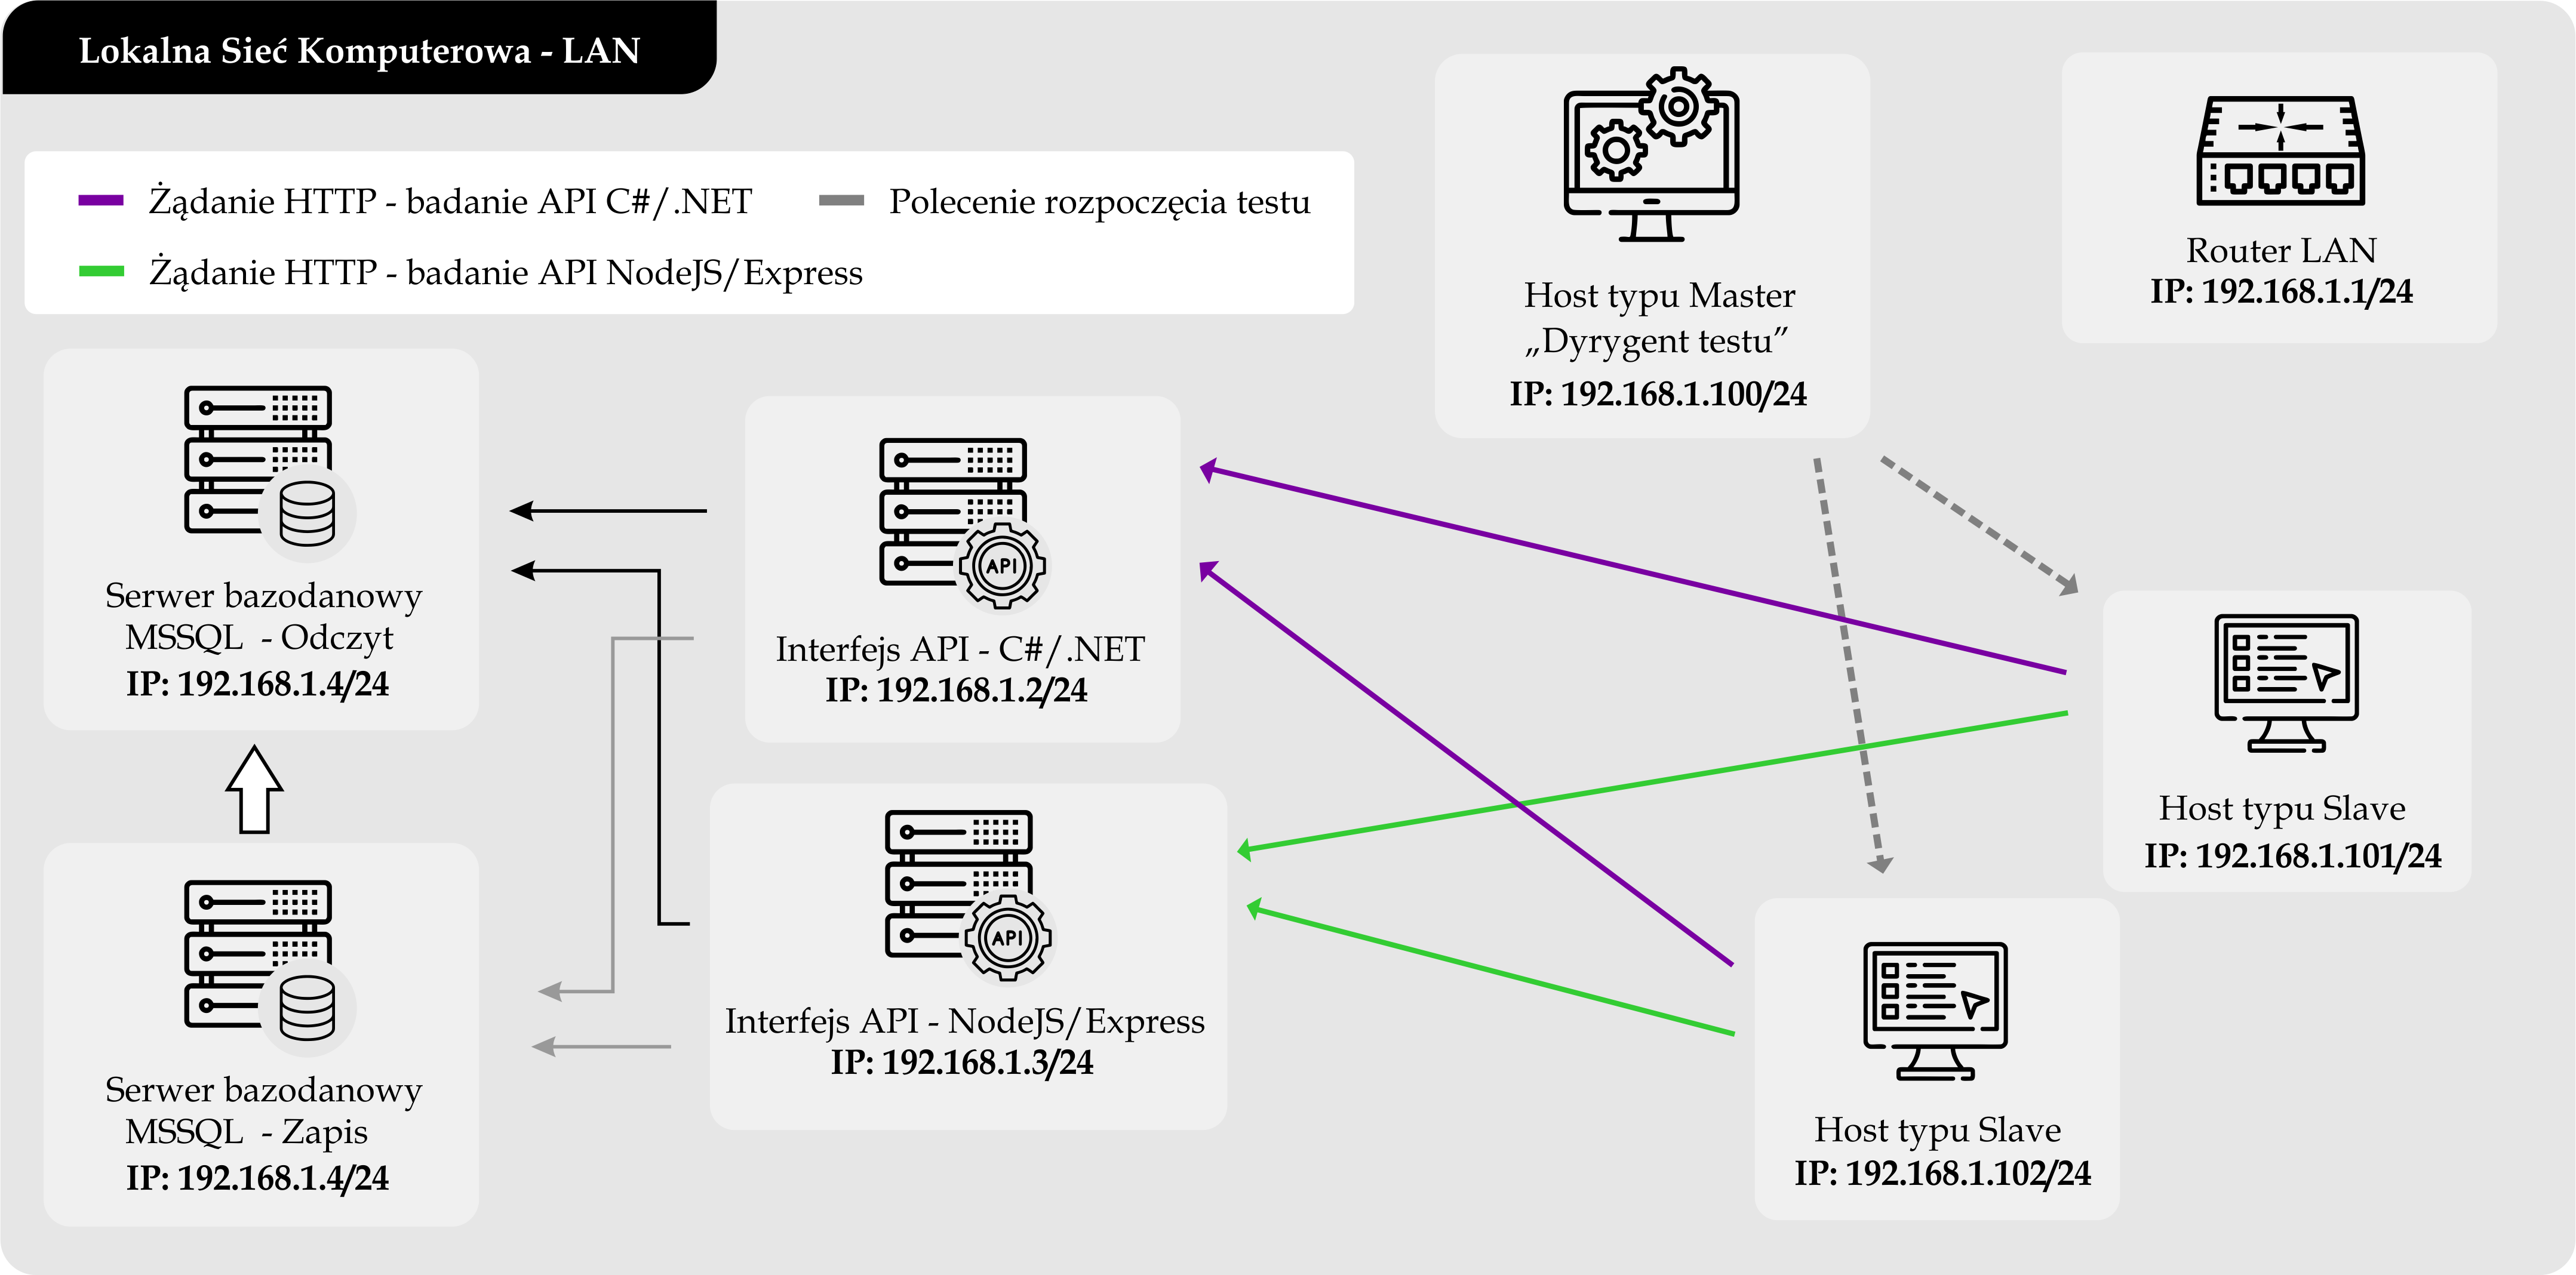
\includegraphics[width=\linewidth]{rys04/topologia-5.png}
    \caption{Konfiguracja czwarta lokalnej topologii fizycznej środowiska badawczego}
    \label{fig:topologia-5}
\end{figure}

\subsection*{Konfiguracja pierwsza rozległej topologii fizycznej środowiska badawczego}
\label{sec:rozproszone-srodowisko-badawcze-ver-1}
Konfiguracja topologii fizycznej dla rozproszonego środowiska badawczego, stworzona została w celu wykonania badań dotyczących efektywności działania interfejsów programowania aplikacji uruchamianych na odmiennych platformach chmurowych.

W tym przypadku, wyodrębnić należy dwa obszary, zawierające urządzenia w kontekście których przeprowadzana jest ewaluacja. Pierwszy obszar to lokalna sieć komputerowa, w której ulokowane zostały urządzenia końcowe odpowiedzialne za przechowywanie konfiguracji badania, a także generowanie żądań w kierunku API. W drugim obszarze zaś, nazwanym rozległą siecią komputerową uruchomione są platformy chmurowe, wewnątrz których działają interfejsy programowania aplikacji oraz serwery bazodanowe. Systemy internetowe zaimplementowane w odrębnych technologiach, przechowywane są na oddzielnych platformach chmurowych i nie są one ze sobą w żaden sposób skomunikowane. Zauważyć należy również fakt, że obie platformy chmurowe znajdują się w różnych lokalizacjach geograficznych. Stwierdzenia te, wymuszają modyfikację sposobu pozyskiwania pomiarów żądań, poprzez przeniesienie odpowiedzialności za wyliczenie czasu wykonywania operacji na interfejsy programowania aplikacji. Pomimo tego, niezbędnym jest posiadania urządzenia generującego żądania zgodnie z określoną charakterystyką. Dlatego też, wewnątrz obszaru lokalnego wskazać możemy dwa urządzenia końcowe, których rolą, podobnie do urządzeń końcowych zawartych we wszystkich poprzednich topologii fizycznych, jest generowanie żądań, oraz koordynowanie przeprowadzanego badania.

Na ilustracji \ref{fig:topologia-4} przedstawiono schemat pierwszego wariantu rozległej topologii fizycznej środowiska badawczego.

\begin{figure}[ht]
    \centering
     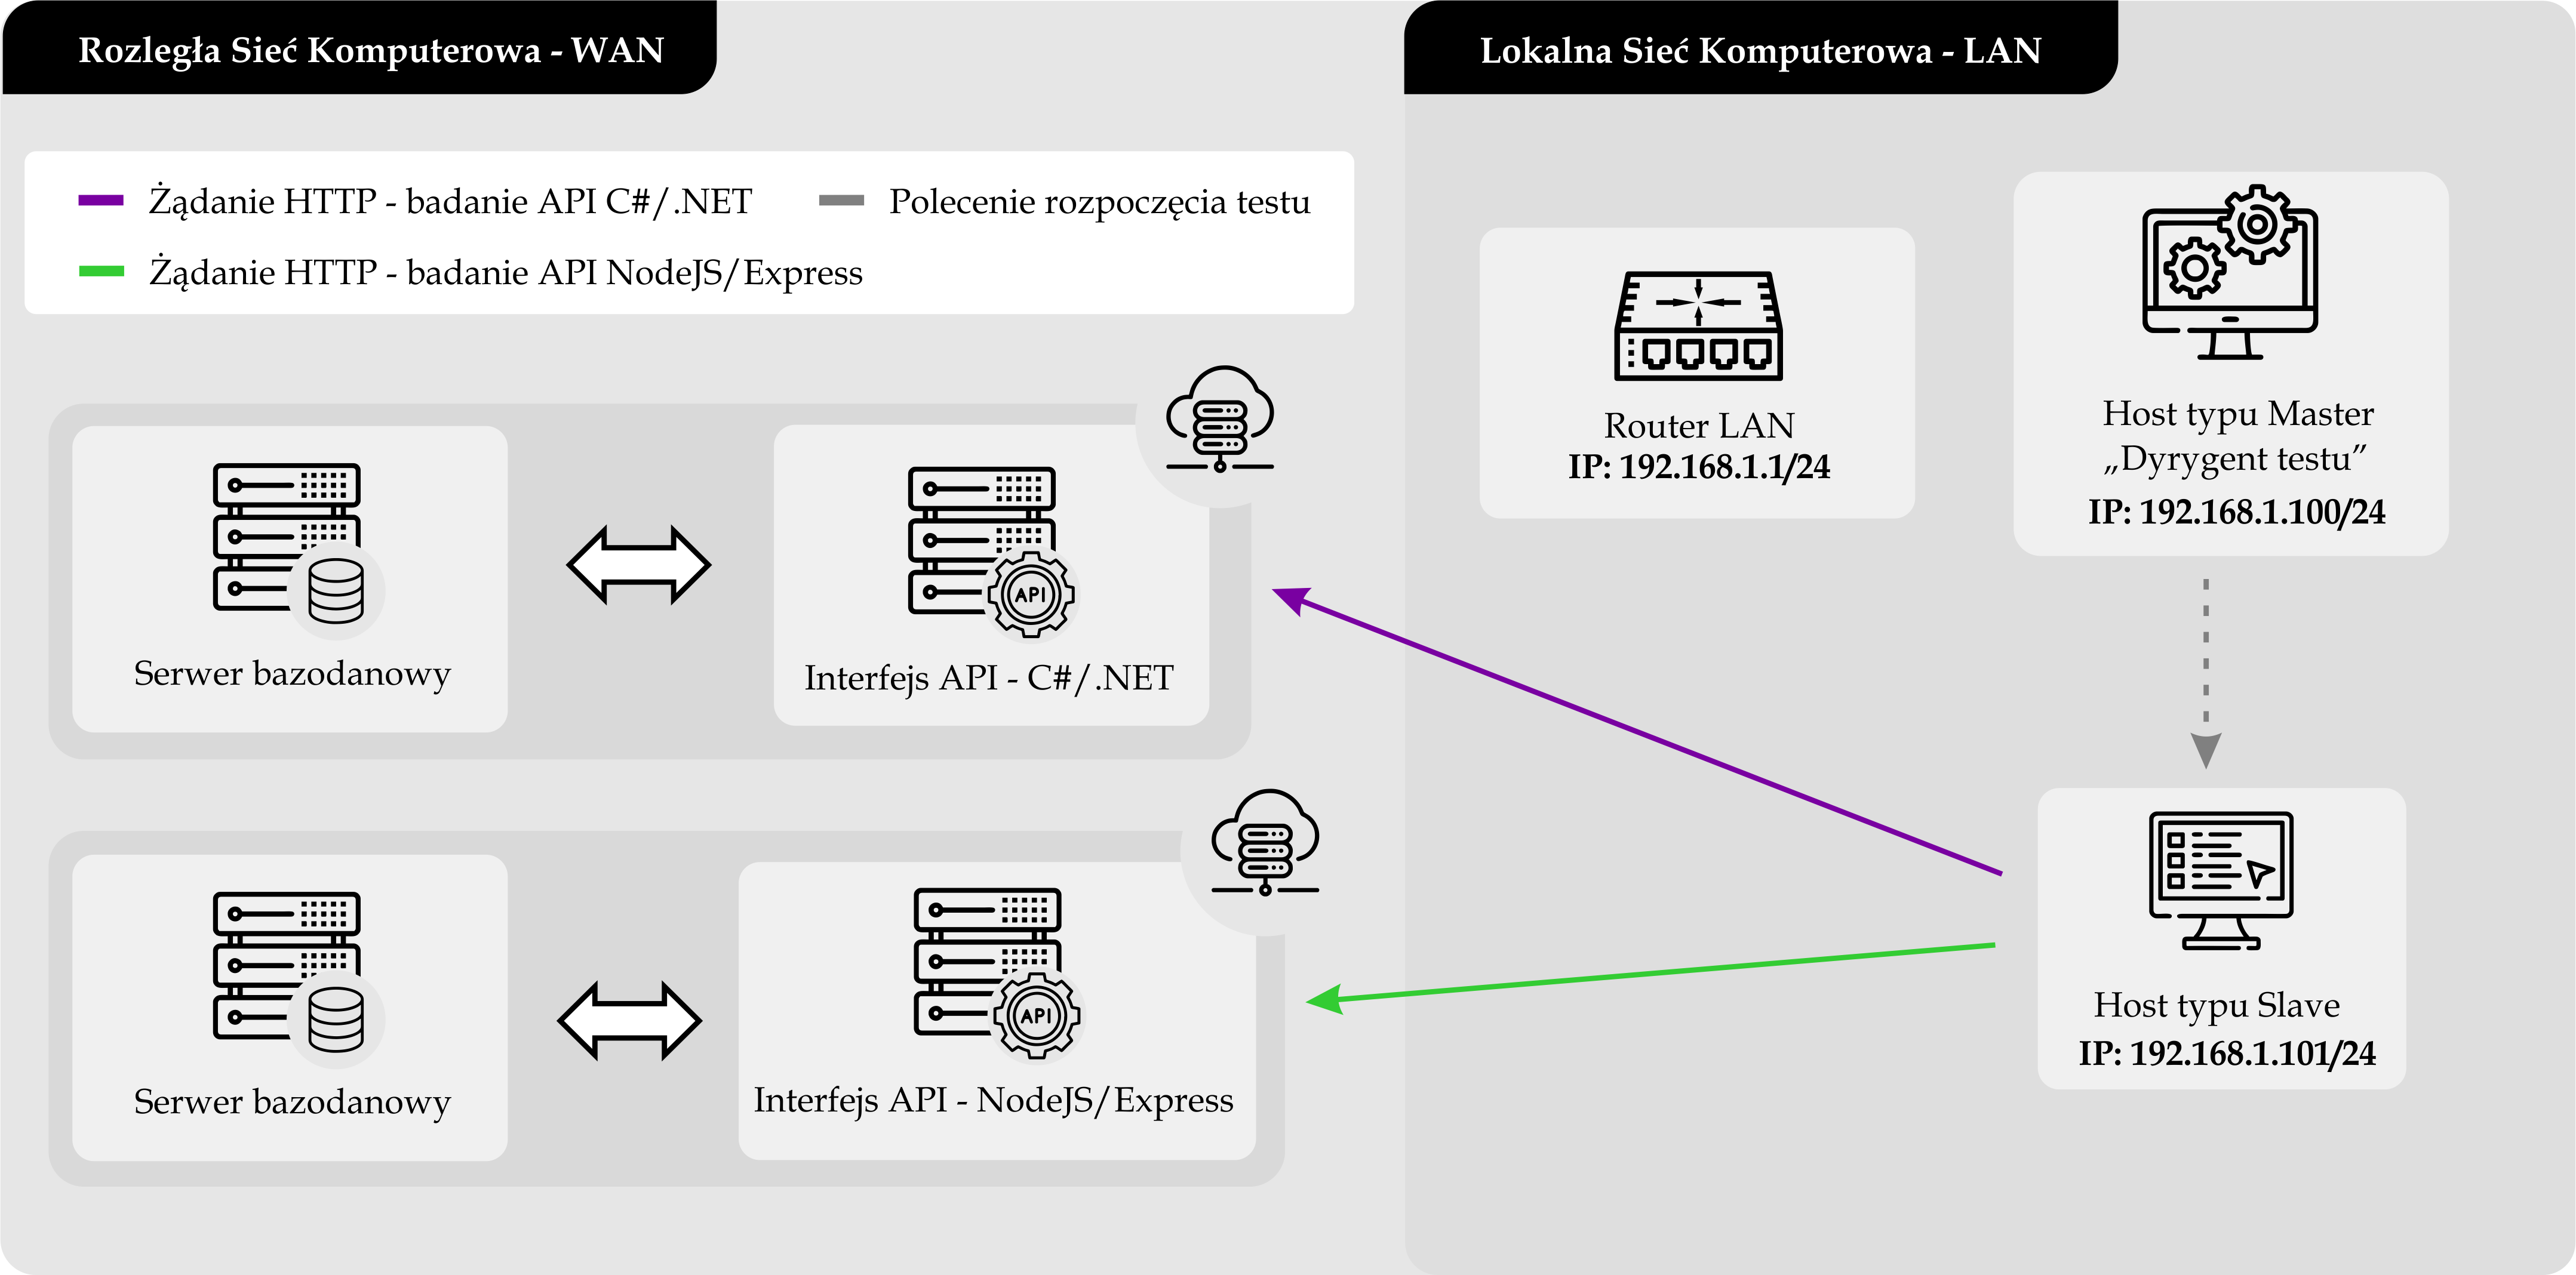
\includegraphics[width=\linewidth]{rys04/topologia-4.png}
    \caption{Konfiguracja pierwsza rozległej topologii fizycznej środowiska badawczego}
    \label{fig:topologia-4}
\end{figure}

\section{Budowa interfejsów programowania aplikacji}
\subsection*{Ogólna funkcjonalność interfejsów programowania aplikacji}
Niezależnie od rozważanej technologii, interfejsy programowania aplikacji implementowane w celu przeprowadzania badań zawartych w ramach niniejszej pracy magisterskiej, dostarczają funkcjonalności obsługi lokalu restauracyjnego. W obrębie omawianych aplikacji zdefiniować można konta użytkowników należących do jednej z pięciu ról pracowniczych. Wyróżnić należy stanowiska: administratora systemu, zarządcy przedsiębiorstwem, kierownika sali, kucharza, a także kelnera. Użytkownicy dysponujący jedną z wymienionych ról mogą korzystać z określonego zestawu funkcjonalności, który determinowany jest poziomem uprawnień zależnych od stanowiska. Przed wywołaniem funkcjonalności systemu, każdy z użytkowników musi zostać uwierzytelniony, a także autoryzowany. Uwierzytelnienie polega na odwołaniu się do punktu końcowego logowania i podaniu swoich danych poświadczeń. Jeżeli dane poświadczeń wskazują na konkretnego użytkownika API, w odpowiedzi zwracany jest token uwierzytelniający, który musi zostać następnie dołączony do nagłówka każdego z wywoływanych żądań. Proces autoryzacji odbywa się na poziomie funkcji warstwy pośredniczącej \textit{(ang. Middleware)}, tuż przed rozpoczęciem wykonywania kodu metody klasy kontrolera.

W kontekście funkcjonalności tworzonych usług sieciowych wymienić należy:
\begin{itemize}
    \item definiowanie oraz zarządzanie strukturą lokalu restauracyjnego (zarządzanie pomieszczeniami lokalu, określanie układu stolików wewnątrz pojedynczego pomieszczenia)
    \item obsługa procesu zamównienia (zarządzanie rachunkami, daniami, statusami przetwarzania posiłków, a także dyspozycjami klientów)
    \item zarządzanie gospodarką magazynową lokalu restauracyjnego (obserwacja stanów ilościowych w kontekście produktu, obsługa danych produktu, definiowanie kategorii produktowych).
\end{itemize}

Dodatkowe funkcje systemu, nie związane z przeprowadzaniem operacji typu CRUD, takie jak wdrożenie metody wyznaczania trasy dla dostarczania zamówień poprzez implementację algorytmu dla symetrycznego problemu komiwojażera, opisane zostały w następnych sekcjach niniejszego rozdziału.
\subsection*{Interfejs API realizujący operacje CRUD stworzony z wykorzystaniem technologii C\#/.NET}
Omawiany interfejs programowania aplikacji zaimplementowany został w języku C\#, z zastosowaniem środowiska uruchomieniowego .NET w wersji piątej. Usługa sieciowa, o której mowa w niniejszym podrozdziale, stanowi złożenie dwóch składowych. Pierwszą z nich jest program, którego zadaniem jest dostarczenie definicji oraz obsługa określonych poleceń klienta, wydanych w postaci żądań protokołu hipertekstowego. Ściśle rzecz ujmując, to właśnie ten program należy określić terminem interfejsu programowania aplikacji. Jako drugą składową natomiast, wskazać należy serwer warstwy aplikacji, pozwalający na obsługę komunikacji pomiędzy usługą sieciową a urządzeniami z zewnątrz. Serwerem wykorzystanym w ramach zaimplementowanej usługi sieciowej jest otwartoźródłowe oprogramowanie Kestrel.

W celu powiązania metod operujących na wewnętrznym modelu danych z fizycznymi strukturami bazodanowymi wykorzystano maper obiektowo-relacyjny Entity Framework Core w wersji drugiej dla relacyjnych systemów baz danych, a także narzędzie Mongoose dla nierelacyjnej bazy danych MongoDB.

Utworzone w języku C\# rozwiązanie złożone jest z pięci projektów powiązanych pomiędzy sobą zależnościami. Pierwszy z projektów zawiera klasy kontrolerów, dokumenty json globalnych właściwości usługi w określonych środowiskach, punkt startowy programu, a także klasę konfiguracji dla wszystkich definiowanych w obrębie całego rozwiązania usług. W projekcie tym, można uzyskać dostęp do struktur programistycznych, definiowanych we wszystkich pozostałych fragmentach rozwiązania.

Drugi z projektów, stworzony został z myślą przechowywania kodu źródłowego związanego z przetwarzaniem logiki biznesowej programu. Zdefiniowane zostały tu klasy serwisów, metody rozszerzeń dla typów języka, obiekt parametrów paginacji, klasy transferu danych \textit{(ang. Data Transfer Objects)}, a także prodecury generowania opowiedzi dla użytkownika. Od projektu tego, zależne są wszystkie fragmenty rozwiązania z wyłączeniem pierwszego z omawianych.

Na równorzędnym poziomie hierarchii, zdefiniowany został projekt dotyczący obsługi operacji związanych z bezpieczeństwem interfejsu API. Wyróżnić możemy tutaj klasę generatora tokenu uwierzytelniającego, a także metodę dostępu do właściwości identyfikujących użytkownika poprzez zawartość kontekstu żądania http.

Kolejnym fragmentem rozwiązania stworzonego w języku C\# jest projekt dostępu do danych. W projekcie tym, wskazać należy klasę kontekstu danych, zbiór migracji modelu danych do schematów bazodanowych, klasę propagacji danych początkowych, a także listę metod struktur repozytoriów, które pozwalają na wykonywanie bezpośrednich operacji na wykorzystywanym zbiorze informacji. Omawiany fragment, posiada zależność względem projektu logiki biznesowej.

Ostatnim projektem rozwiązania jest przestrzeń przechowywania klas modelu danych. Fragment ten, nie wprowadza zależności względem jakiegokolwiek z pozostałych projektów i pełni rolę rdzenia aplikacji. Każda z omówinionych powyżej przestrzenii kodu źródłowego posiada dostęp do elementów modelu, jednakże jakiekolwiek operacje na tych danych, wykonywane są tylko i wyłącznie z poziomie klas repozytoriów.

Na ilustracji \ref{fig:struktura-plikow-dotnet} przedstawiono strukturę obiektów wewnątrz poszczególnych fragmentów rozwiązania. Niektóre spośród elementów każdego projektu zostały pominięte na niniejszym rysunku w celu zachowania czytelności omawianej treści.

\begin{figure}[ht]
    \centering
     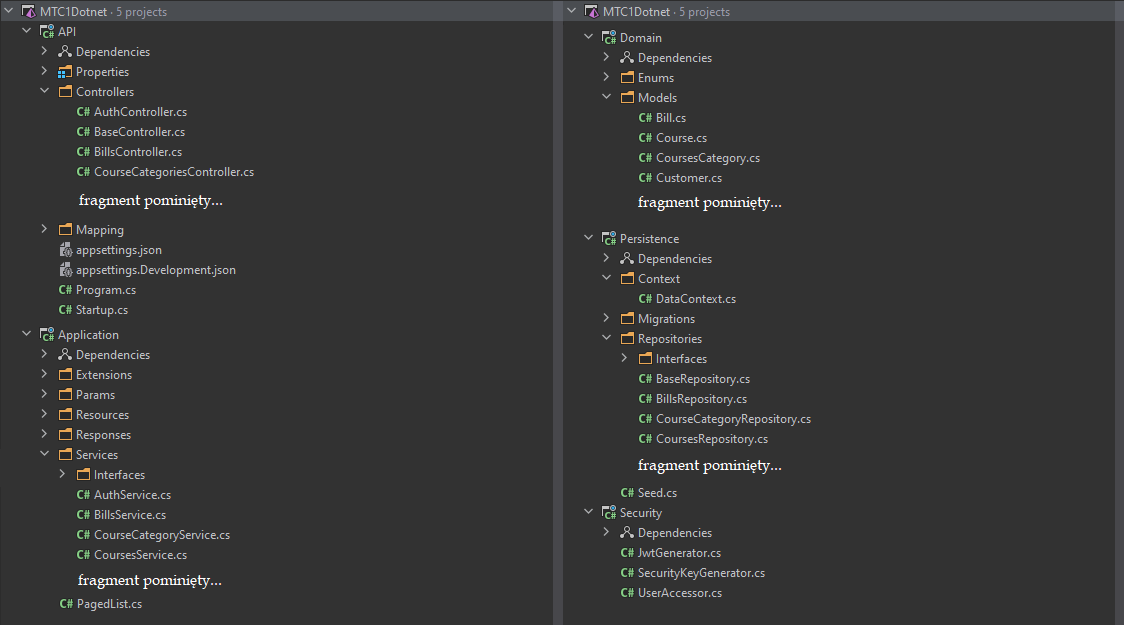
\includegraphics[width=\linewidth]{rys04/struktura-plikow-dotnet.png}
    \caption{Struktura obiektów wewnątrz rozwiązania systemu internetowego zaimplementowanego w języku C\#}
    \label{fig:struktura-plikow-dotnet}
\end{figure}
\subsection*{Interfejs API realizujący operacje CRUD stworzony z wykorzystaniem technologii NodeJS/Express}
Druga z realizacji interfejsu programowania aplikacji napisana została w języku JavaScript, zgodnym ze specyfikacją językową ECMAScript 6. Do implementacji funkcjonalności omawianej usługi sieciowej, wykorzystano bibliotekę ExpressJS w wersji czwartej, a całość oprogramowania uruchomiono na serwerze wykorzystującym natywne moduły platformy uruchomieniowej NodeJS.

W celu powiązania metod operujących na wewnętrznym modelu danych z fizycznymi strukturami bazodanowymi wykorzystano maper obiektowo-relacyjny Prisma w wersji pierwszej dla relacyjnych systemów baz danych, a także narzędzie Mongoose dla nierelacyjnej bazy danych MongoDB.

W przeciwieństwie do rozwiązania utworzonego przy wykorzystaniu technologii firmy Microsoft, schemat struktur programistycznych interfejsu programowania aplikacji opartego o JavaScript cechuje się znacząco niższym poziomem skomplikowania. Całość oprogramowania przechowywana jest w ramach pojedynczego projektu, wewnątrz którego podział struktur programistycznych ze względu na odpowiedzialności dokonany został na poziomie folderów.

Punktem startowym aplikacji, a także miejscem definicji podstawowej konfiguracji elementów usługi sieciowej jest skryptowy plik o nazwie \textit{app.js}. W pliku tym, określono wartości dla zmiennych globalnych dotyczących ścieżki podstawowej w aplikacji, czy też klucza tajnego wykorzystywanego do wyliczania tokenu uwierzytelniania. Ponadto, określono funkcje pośredniczące wykonujące się przed rozpoczęciem zadanej funkcji modułu kontrolera. Plik \textit{app.js}, zawiera także informacje dotyczące lokalizacji modułów, odpowiadających za obsługę punktów końcowych dla określonej ścieżki wywołania.

Poza plikiem startowym interfejsu programowania aplikacji wskazać należy foldery, przechowujące moduły odpowiedzialne za poprawną pracę całości aplikacji. Pierwszy z folderów o nazwie \textit{controllers}, stanowi zbiór modułów zawierających funkcje obsługujące każdy z zaimplementowanych punktów końcowych. Funkcje te, odwołują się do fragmentów oprogramowania realizujących operacje logiki biznesowej, które to fragmenty umieszczone są w folderze \textit{services}. Analogiczne odwołanie ma miejsce w kontekście modułów serwisów a funkcji operujących na danych. Funkcje te, znaleźć można w folderze \textit{repositories}. Ponadto, wyróżnić należy katalog \textit{errors}, przechowujący kod źródłowy dotyczący przetwarzania błędów dla każdej z logicznych warstw interfejsu, katalog \textit{helpers} w ramach którego zdefiniowane zostały funkcje pomocnicze, a także folder \textit{prisma}, zawierający w sobie pliki migracji oraz dokument definicji schematu modelu danych.

Na ilustracji \ref{fig:struktura-plikow-nodejs} przedstawiono strukturę obiektów wewnątrz poszczególnych fragmentów rozwiązania. Niektóre spośród elementów każdego projektu zostały pominięte na niniejszym rysunku w celu zachowania czytelności omawianej treści.

\begin{figure}[ht]
    \centering
     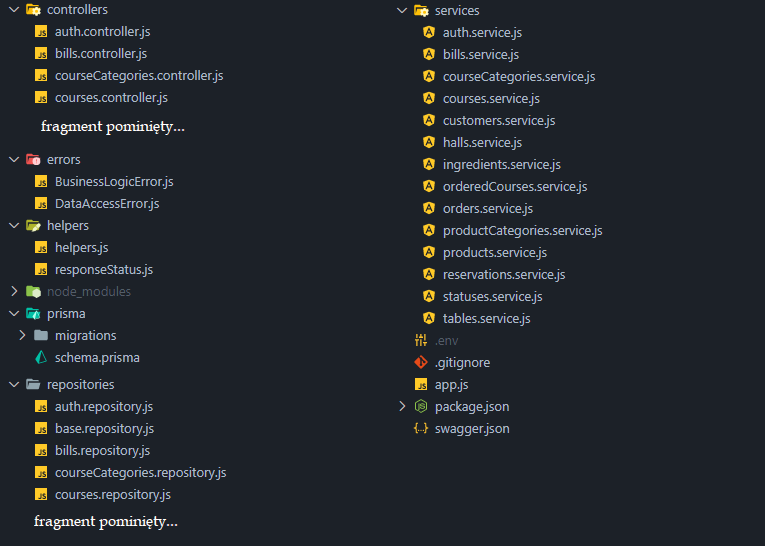
\includegraphics[width=\linewidth]{rys04/struktura-plikow-nodejs.png}
    \caption{Struktura obiektów wewnątrz rozwiązania systemu internetowego zaimplementowanego w języku JavaScript}
    \label{fig:struktura-plikow-nodejs}
\end{figure}

\subsection*{Algorytm metaheurystyczny dla symetrycznego problemu komiwojażera}
W celu realizacji badania wydajności przetwarzania operacji współbieżnych zdecydowano się na implementację algorytmu metaheurystycznego przeznaczonego do rozwiązywania symetrycznego problemu komiwojażera. Zaimplementowany algorytm, sklasyfikować należy jako heurystykę z rodziny algorytmów genetycznych. Algorytmy te, zaliczane są do przestrzenii schematów ewolucyjnych, których główną koncepcją jest próba przeniesienia procesów, a także zachowań biologicznych obserwowanych w ramach dziedziny genetyki, w obszar definiowania oraz realizacji algorytmów. 

Należyte przedstawienie procesu wykonania algorytmu genetycznego wymaga wprowadzenia odpowiedniej terminologii. Terminologia ta, podobnie jak wspomniane uprzednio obserwowane procesy biologiczne, została zaczerpnięta z dziedziny genetyki. Podstawowym pojęciem, który należy wyróżnić w ramach wprowadzanych definicji jest chromosom. W kontekście algorytmu genetycznego jest on iterpretowany jako pojedynczy element rozwiązania określonego problemu optymalizacyjnego (w tym przypadku, pojedyncza lokalizacja która ma zostać odwiedzona przez osobę przemierzającą trasę). Wszystkie spośród permutacji zbioru chromosomów, przy założeniu, że liczba elementów permutacji równa jest wielkości zbioru, identyfikowane są jako osobniki, w ramach określonej populacji. Każdy z osobników populacji może zostać poddawany modyfikacji jego kodu genetycznego (zmiany jego chromosomów), poprzez zdefiniowane operacje krzyżowania osobników, a także ich mutacji. Ponadto, w celu wyboru najlepszych spośród osobników, wykonywany jest proces selekcji. Proces ten, powiązany jest ściśle z metryką oceny jakości osobnika względem populacji nazywaną funkcją przystosowania.

Na rysunku \ref{fig:algorytm-genetyczny} zilustrowano schemat blokowy algorytmu genetycznego.

\begin{figure}[ht]
    \centering
     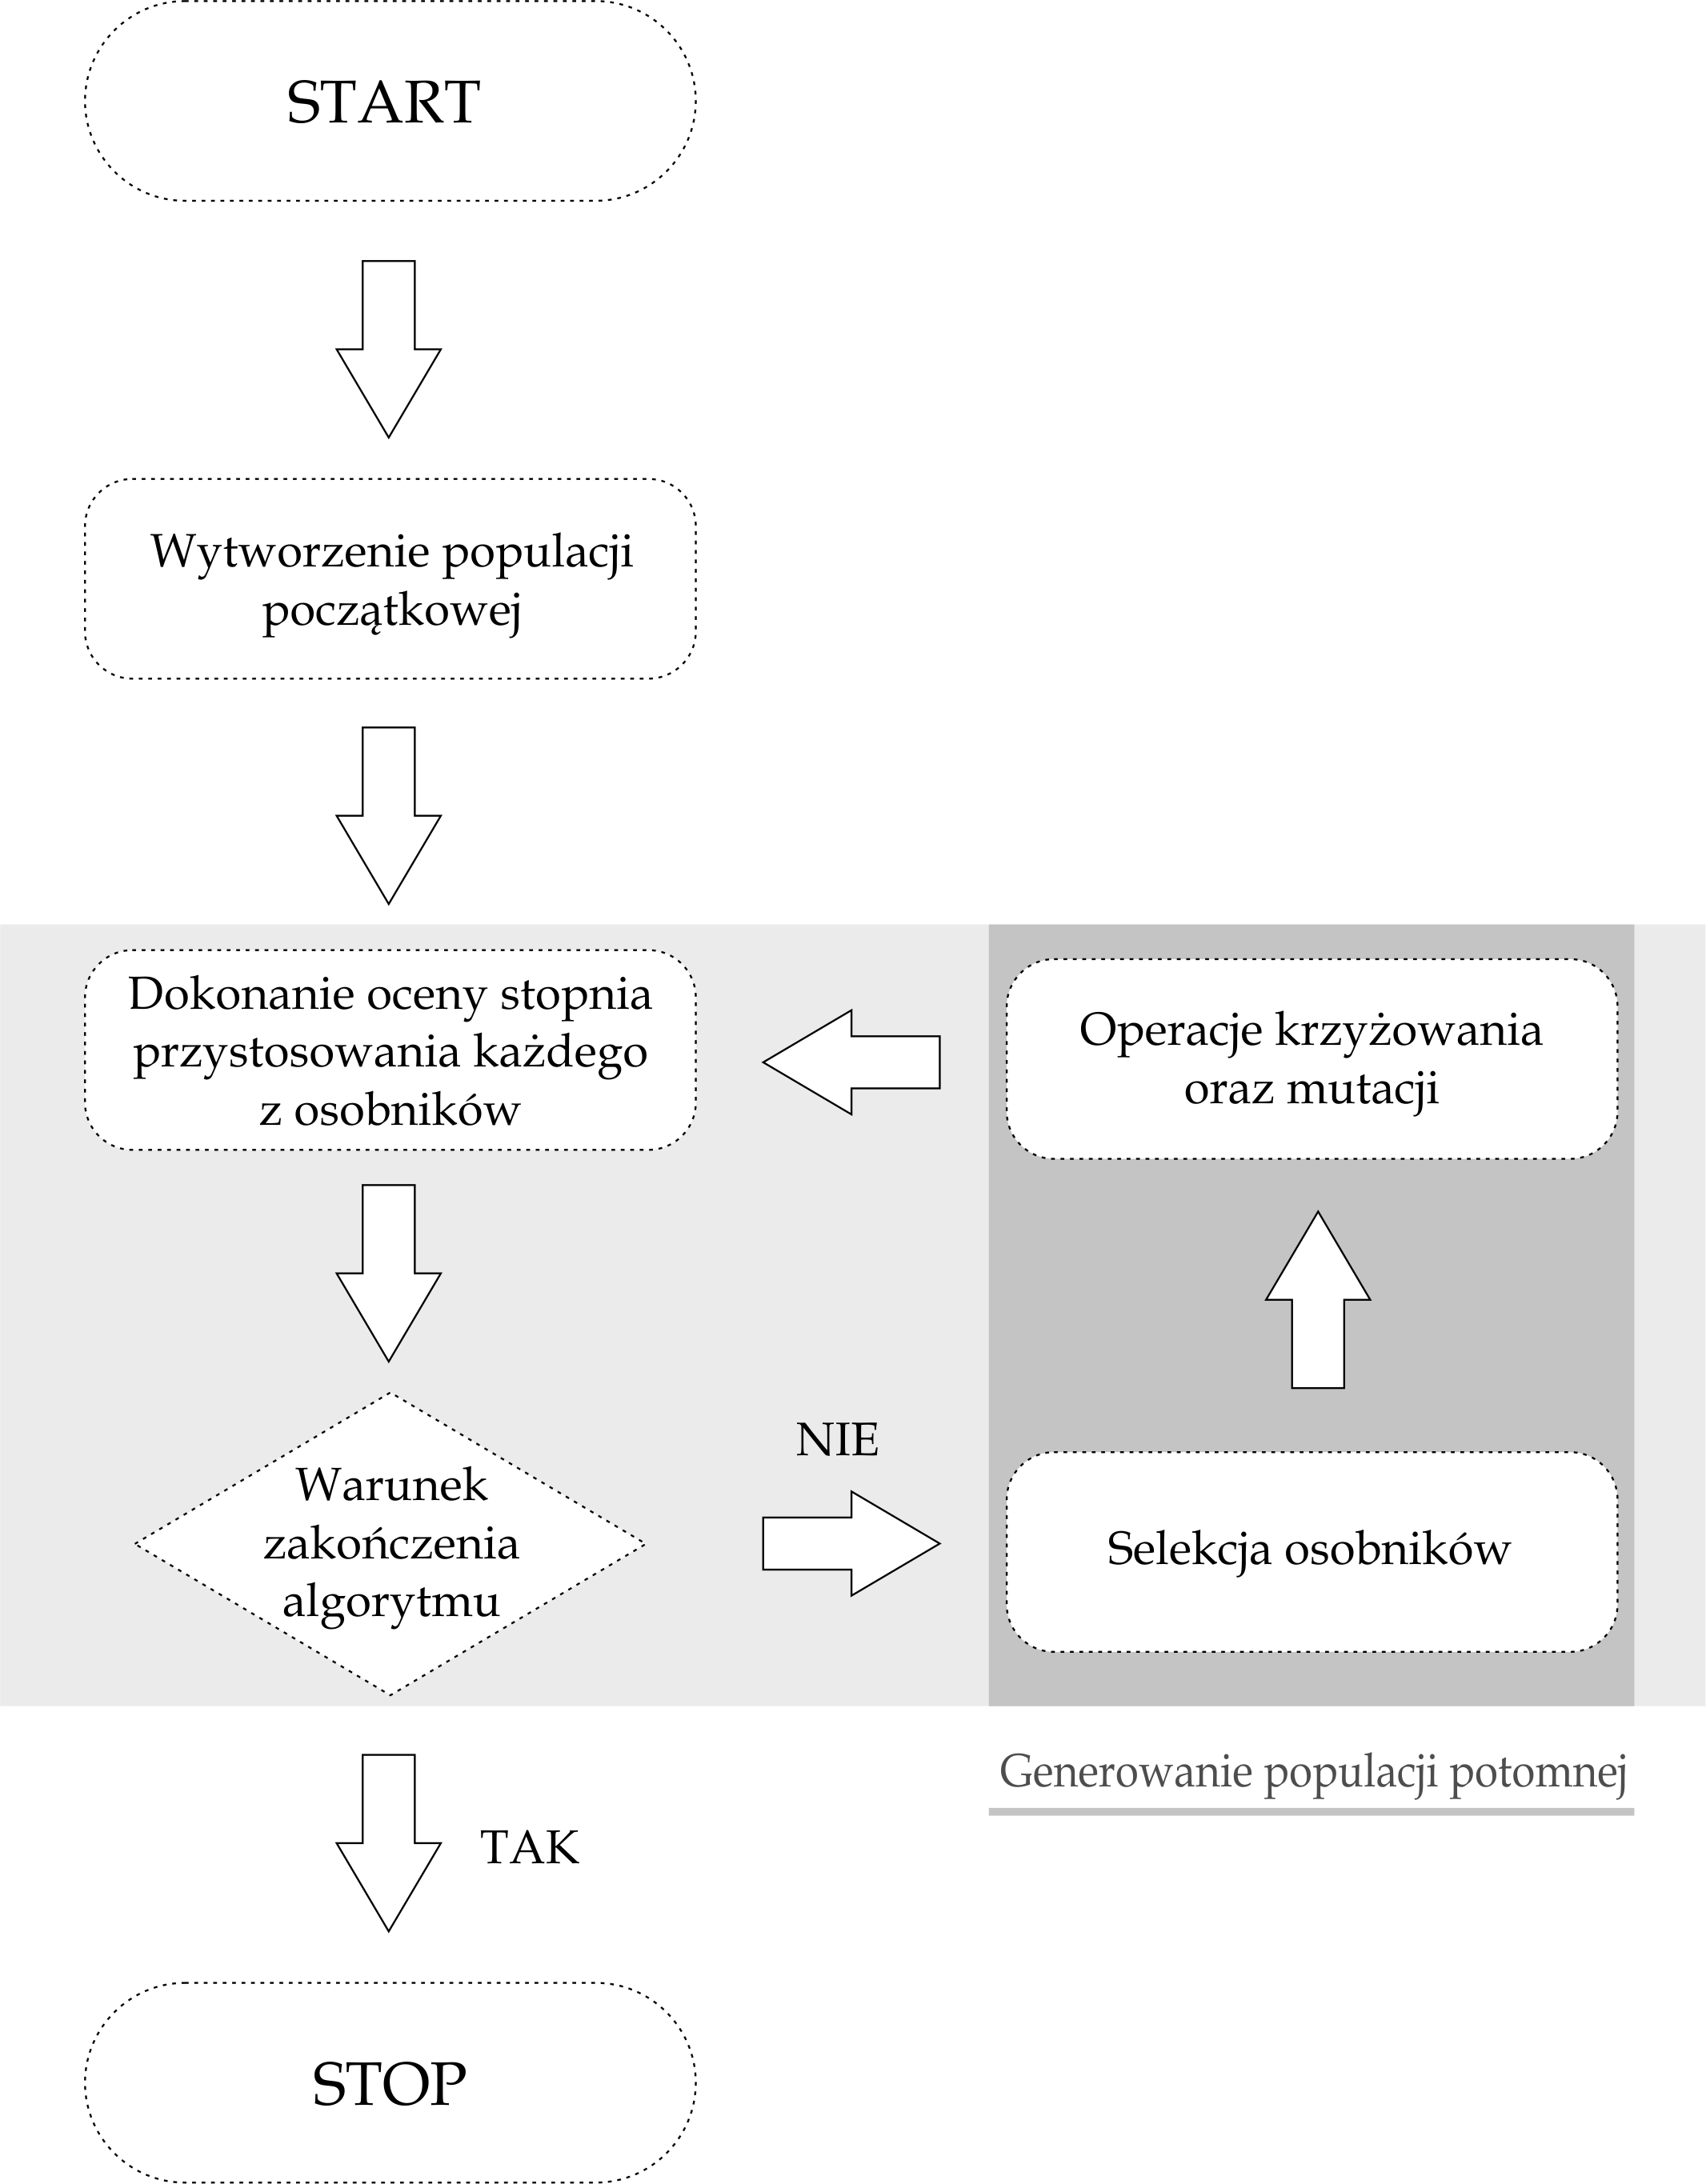
\includegraphics[width=0.6\linewidth]{rys04/algorytm-genetyczny.png}
    \caption{Schemat blokowy algorytmu genetycznego}
    \label{fig:algorytm-genetyczny}
\end{figure}

Implementowane rozwiązanie omawiane w ramach niniejszej pracy dyplomowej cechuje się realizacją funkcji krzyżowania osobników z wykorzystaniem dwóch punktów podziału (tzw. krzyżowanie dwupunktowe), a także dokonaniem mutacji w zależności od przyjętego prawdopodobieństwa. Ponadto, metodę selekcji oparto na technice ruletkowej, wzbogacają technikę tę, o mechanizm zapobiegania zjawisku przedwczesnej zbieżności poprzez kontrolę liczby osobników dominujących w populacji.

W tabeli \ref{tab:hiperparametry-genetyczny} wymieniono hiperparametry zaimplementowanej metaheurystyki genetycznej, a także opisano ich znaczenie w kontekście schematu działania algorytmu.

\begin{table}[htbp] \small
\centering
\caption{Wykaz hiperparametrów zaimplementowanego algorytmu genetycznego}
\label{tab:hiperparametry-genetyczny}
\begin{tabularx}{\linewidth}{|X|X|X|} \hline\
    Nazwa parametru & Opis & Wartość domyślna \\ \hline\hline
    Prawdopodobieństwo mutacji osobnika & Parametr definiujący częstość wystąpienia zdarzenia modyfikacji pojedynczego chromosomu w obrębie osobnika & 0,01 \\ \hline
    Prawdopodobieństwo krzyżowania osobników & Parametr definiujący częstość wystąpienia zdarzenia wymiany kodu genetycznego pomiędzy określonymi osobnikami & 1 \\ \hline
    Rozmiar populacji & Liczba osobników poddawanych ewolucji, spośród których ostatecznie wybierane jest rozwiązanie najlepsze & 0,75 * liczba wszystkich rozpatrywanych lokalizacji \\ \hline
    Liczba osobników dominujących w ramach pojedynczej populacji & Rozmiar podgrupy w obrębie pojedynczej populacji, skupiającej w sobie osobników o najwyższych wartościach funkcji przystosowania & 0.25 * rozmiar populacji \\ \hline
    Czas wykonania algorytmu & Przedział czasu określany przez liczbę sekund, w ramach którego wykonywana będzie główna pętla algorytmu & 60 \\ \hline
\hline
\end{tabularx}
\end{table}

Niezależnie od środowiska, w którym implementowany został opisany powyżej algorytm, sposób uruchamiania, przekazywania danych wejściowych, a także format danych wyjściowych jest identyczny. Omawiany algorytm metaheurystyczny dostępny jest z poziomu punktu końcowego określonych interfejsów programowania aplikacji jako żądanie protokołu hipertekstowego dla ścieżki \textit{/api/algorithms/roadPlan} oraz metody HTTP POST. Format danych wejściowych określony został jako tablica obiektów notacji JSON, zawierających właściwości definiujące szerokość i długość geograficzną, a także adres dla pojedynczej lokalizacji. Rezultatem otrzymywanym w ramach odpowiedzi protokołu hipertekstowego jest obiekt zawierający informacje dotyczącą ilorazu uzyskanego wyniku względem wyniku optymalnego, a także liczbę przeprowadzonych w pętli głównej algorytmu. Czas wykonania pojedynczego żądania dla omawianego punktu końcowego wynosi co najmniej 60 sekund.


W odniesieniu do szczegółów implementacyjnych tyczących się języka C\# oraz środowiska uruchomieniowego .NET, wspomnieć należy o wykonaniu kodu źródłowego głównej pętli algorytmu w ramach osobnego wątku. Po zdefiniowaniu wartości hiperparametrów heurystyki, inicjowana jest nowa instancja klasy \textit{Thread}, która przyjmuje w ramach konstruktora metodę wykonawczą (w tym przypadku metodę pętli głównej algorytmu). Następnie, obiekt klasy \textit{Timer}, odlicza czas 60 sekund, w ramach których pętla programu może być wykonana. Po upłynięciu czasu wykonania kodu, wątek algorytmiczny łączony jest z głównym wątkiem wykorzystywanym do przetwarzania żądania, a rezultaty działania algorytmu formułowane są do postaci ciała odpowiedzi protokołu HTTP.  


W ramach interfejsu programowania aplikacji zaimplementowanego w języku JavaScript, sposób przetwarzania współbieżnego różni się w sposób znaczący względem języka C\#. Język JavaScript jest rozwiązaniem które dostarcza mechanizmy przetwarzania tylko i wyłączenie w obrębie pojedynczego wątku procesora. Dlatego też, wspominając o tej właśnie technologii programistycznej nie można stwierdzić, że istnieje możliwość współbieżnego wykonania kodu źródłowego. Przepływ sterowania od momentu wywołania punktu końcowego uwzględnia inicjalizację serwisu realizacji algorytmów, zdefiniowanie hiperparametrów programu, rozpoczęcie wykonania pomiaru czasu, a także uruchomienie pętli głównej algorytmu. Pomiar czasu wykonywany jest za pomocą natywnej struktury programistycznej dostarczanej zarówno w ramach środowiska NodeJS, jaki i implementowanej przez silniki obsługi języka JavaScript w przeglądarkach internetowych (tj. interfejs \textit{Performance}).
\subsection*{Mechanizmy obsługi pamięci podręcznej}
Implementacja mechanizmów obsługi pamięci podręcznej wykonana została w oparciu o otwartoźródłowe rozwiązanie \textit{Redis}, dostarczające zarówno strukturę danych pełniącą rolę magazynu wpisów pamięci cache, jak i interfejsy programistyczne służące do ustanowienia połączenia, a także zarządzania zawartością tej struktury. Magazyn pamięci podręcznej Redis uruchomiony został jako autonomiczna usługa sieciowa poprzez wykonanie obrazu \textit{bitnami/redis} w obrębie kontenera \textit{Docker}.

Niezależnie od badanej technologii programistycznej, zaimplementowane mechanizmy pamięci podręcznej są niezależne od określonego punktu końcowego i mogą zostać połączone z dowolną metodą klasy kontrolera, której wynikiem działania jest obiekt odpowiedzi, specyficzny względem wybranego języka. Wykonanie kodu źródłowego związanego z obsługą mechanizmów pamięci podręcznej odbywa się wewnątrz metod pośredniczących \textit{(ang. Middleware)}. Metody te, uzyskują dostęp zarówno do treści żądania wygenerowanego przez aplikację kliencką, jak i odpowiedzi będącej rezultatem działania metody klasy kontrolera. Implikuje to możliwość definiowania identyfikatorów wpisów w pamięci podręcznej dla każdego z wywołanych żądań.

Klucze poszczególnych elementów przechowywanych w pamięci cache składają się ze składowej ścieżki, oraz składowych parametrów. Każdy z fragmentów identyfikatora wpisu rozdzielony jest znakiem średnika, natomiast w obrębie składowej parametru klucz odseparowany jest od wartości znakiem kreski pionowej. Aby zapewnić jednoznaczność wpisu niezależnie od kolejności w jakiej aplikacja kliencka definiuje parametry wewnątrz ciała żądania, poszczególne składowe właściwości są sortowane w kolejności rosnącej według nazwy parametru.

Na ilustracji \ref{fig:cache-klucz} zaprezentowano format klucza wpisu przechowywanego w pamięci podręcznej.

\begin{figure}[ht]
    \centering
     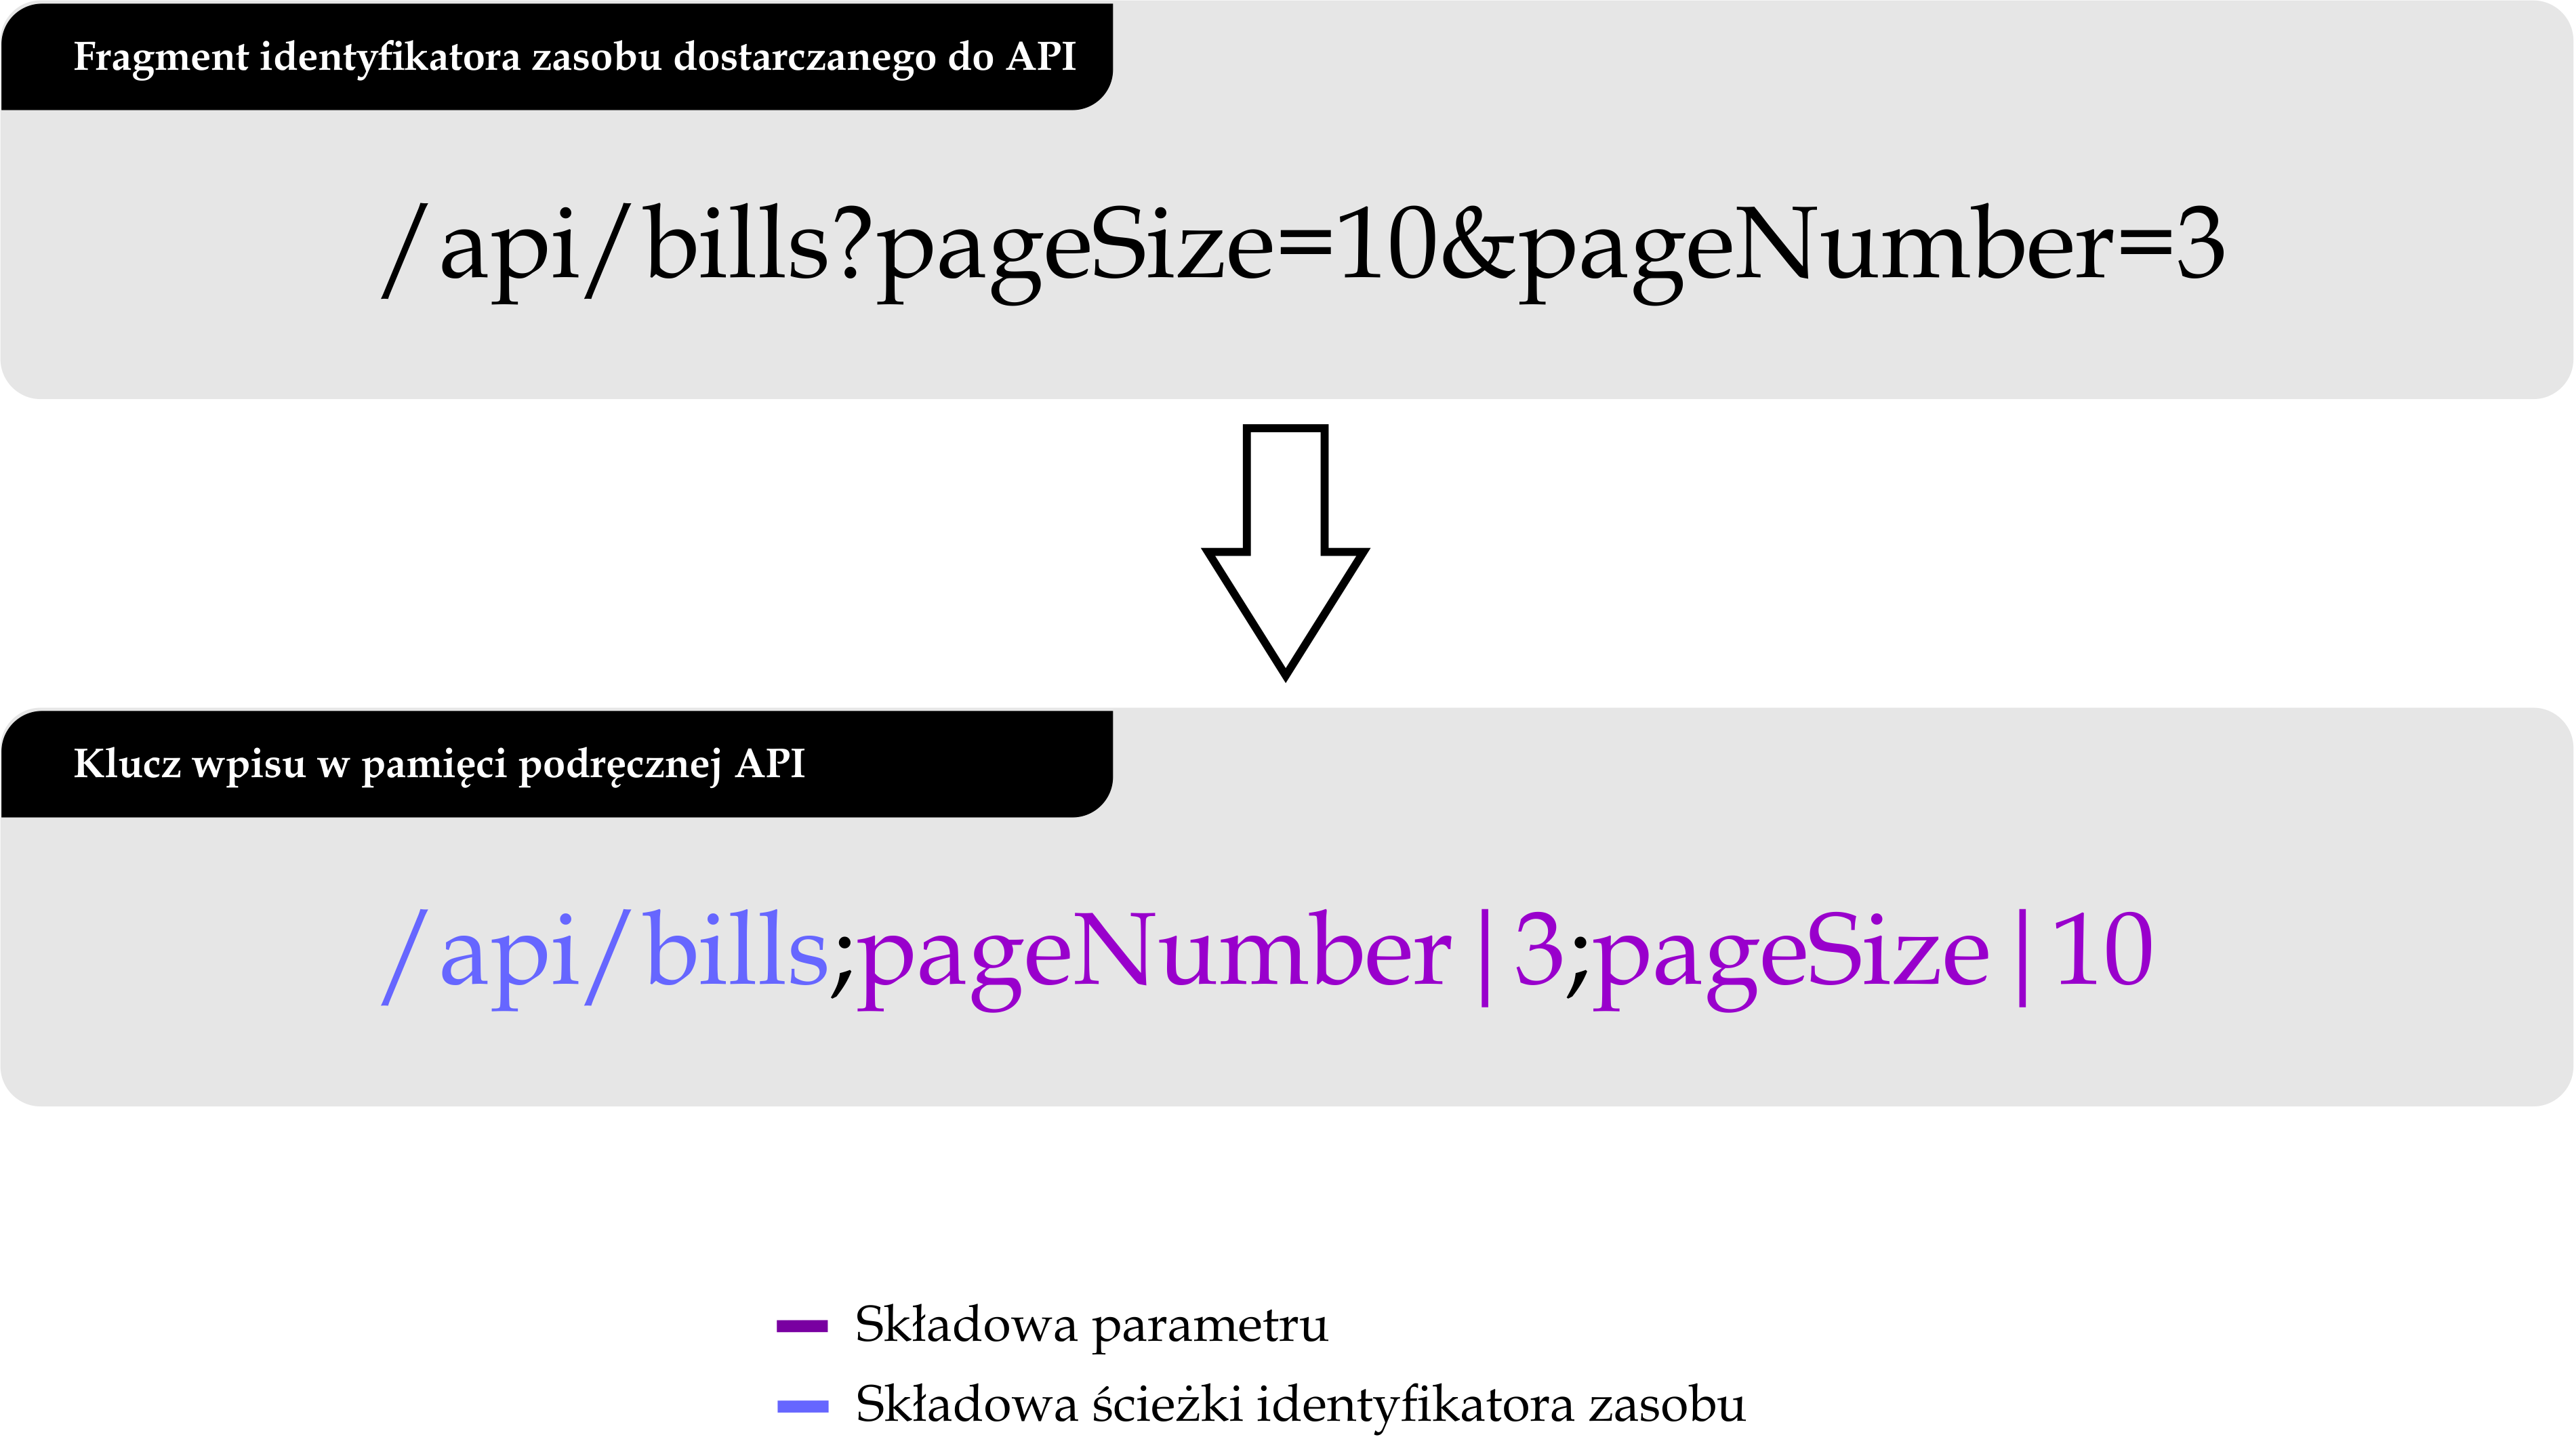
\includegraphics[width=\linewidth]{rys04/cache-klucz.png}
    \caption{Format klucza wpisu przechowywanego w pamięci podręcznej}
    \label{fig:cache-klucz}
\end{figure}

Wdrożone zostały dwa rodzaje mechanizmów obsługi pamięci podręcznej. Pierwszy z nich, zakłada stały czas przechowywania wpisu w magazynie, a także unieważnienie elementu w momencie wywołania metody aktualizacji danych powiązanych z encją opisującą określony element. Mechanizm ten, stanowi klasyczną implementację pamięci podręcznej stosowaną w większości produkcyjnych interfejsów programowania aplikacji.

Drugi mechanizm natomiast, stanowi autorskie podejście twórcy pracy do zarządzania wpisami pamięci podręcznej poprzez ustalenie zmiennego czasu przechowywania elementu w zależności od częstości wywołania punktu końcowego, a także liczby unieważnień. W podejściu tym, wyróżnić należy niezależną strukturę danych, przechowującą liczbę wykonań dla określonego endpointu, a także liczbę wykonań tych punktów końcowych, których działanie prowadzi do unieważnienia wpisu. Przedstawiona struktura jest aktualizowana przy każdym żądaniu wygenerowanym przez klienta i wraz z postępującym działaniem interfejsu programowania aplikacji zawiera coraz bardziej dokładną charakterystykę wywołań poszczególnych obszarów API. Dane te, przechowywane są wewnątrz pamięci programu interfejsu programowania aplikacji, natomiast autor zostawia dowolność co do ich synchronizacji z zewnętrznym źródłem. Synchronizacja ta może być wykonywana poprzez uruchamianie skryptów cyklicznych zadań (np. \textit{cron}), bądź też w momencie uruchamiania oraz wyłączania API.

W momencie tuż przed stworzeniem wpisu i wysyłaniem go do magazynu pamięci podręcznej, w omawianym podejściu następuje kalkulacja czasu życia generowanego elementu. Na początku, obliczany zostaje współczynnik wykonania będący ilorazem liczby uruchomień rozpatrywanego punktu końcowego oraz maksymalnej liczby uruchomień dowolnego z endpointów. Kolejno, w sposób analogiczny tworzony zostaje współczynnik inwalidacji. W tym przypadku stanowi on iloraz wywołań punktów końcowych unieważniających rozpatrywane żądanie i maksymalnej liczby unieważnień dla dowolnego żądania. Oba współczynniki mogą przyjmować wartości z zakresu od zera do jeden. Czas ważności wpisu pamięci podręcznej stanowi iloczyn maksymalnej wartości czasu życia elementu oraz sumarycznego współczynnika wykonania i inwalidacji. Współczynnik ten, określany jest jako suma połowy wartości współczynnika wykonania, a także połowy odwrotności wartości współczynnika unieważnienia. Wprowadzenie takiej formuły prowadzi do uzyskiwania dłuższych czasów przechowywania wpisów dla żądań często wykonywanych oraz rzadko unieważnianych. Wraz ze spadkiem liczby wywołań punktu końcowego, bądź wzrostem liczby jego unieważnień czas ważności wpisu pamięci podręcznej jest zmniejszany. Tak zdefiniowana koncepcja prowadzić powinna do faworyzowania tych punktów końcowych, z których użytkownicy interfejsów korzystają najczęściej.

\begin{equation}
    exec\_factor(x) =  \frac{executions(x)}{max(executions(x):x=1..n)}
    \label{eq:execution-factor}
\end{equation}

\begin{equation}
    invalid\_factor(x) =  \frac{invalidations(x)}{max(invalidations(x):x=1..n)}
    \label{eq:invalidation-factor}
\end{equation}

\begin{equation}
    time\_to\_live(x) = (\frac{1}{2} * exec\_factor(x) + \frac{1}{2} * (1 - invalid\_factor(x))) * max\_time\_to\_live
    \label{eq:time-to-live}
\end{equation}



gdzie:\newline\newline



$executions(x)$ - liczba wywołań punktu końcowego, którego wpis w pamięci podręcznej identyfikowany jest kluczem x \newline\newline
$invalidations(x)$ - liczba unieważnień wpisu pamięci podręcznej identyfikowanego kluczem x \newline\newline
$execution\_factor(x)$ - współczynnik częstości wykonania określonego punktu końcowego \newline\newline
$invalidation\_factor(x)$ - współczynnik częstości unieważnień wpisów dotyczących określonego punktu końcowego \newline\newline
$time\_to\_live(x)$ - czas ważności wpisu dodawanego do pamięci podręcznej \newline\newline
$max\_time\_to\_live(x)$ - maksymalny czas ważności wpisu podręcznej względem którego wyliczany jest faktyczny czas ważności \newline\newline

Kod źródłowy służący do zarządzania elementami pamięci podręcznej zaimplementowany został w API C\# za pomocą funkcji pośredniczących dołączanych do struktur programistycznych w formie atrybutu. Stworzona została klasa dziedzicząca po natywnym typie \textit{Attribute}, a także implementująca interfejs \textit{IAsyncActionFilter}. Implementacja niniejszego interfejsu wymaga zdefiniowania metody \textit{OnActionExecutionAsync}, w ramach której napisano logikę działania obu mechanizmów obsługi cache. Wspomniana metoda, posiada dostęp do kontekstu żądania HTTP przez co możliwe było zarówno wykonanie operacji, tuż przed jak i tuż po uruchomieniu metody klasy konstruktora.

W przypadku platformy uruchomieniowej NodeJS oraz języka JavaScript, wymagane było utworzenie dwóch osobnych funkcji, a także rozdzielenie logiki zarządzania pamięcią podręczną, względem operacji wykonywanych przed oraz po uruchomieniu kontrolera. Interfejs programowania aplikacji tworzony z wykorzystaniem omawianych technologii, a także biblioteki ExpressJS, opiera swoje działanie na ciągu kolejno wywoływanych metod, z których ostatnią jest ta, która wysyła odpowiedź do klienta, korzystając z natywnego obiektu odpowiedzi. Taka zasada działania, wymusiła modyfikację kodu źródłowego metod klas kontrolerów w taki sposób, aby rezultat ich wykonania nie zwracał bezpośrednio odpowiedzi w stronę klienta, a przekazywał ją do kolejnej funkcji pośredniczącej. Stwierdzenie to jednak nie jest sprzeczne z informacją przytoczoną na początku tej sekcji. Chociaż zmieniony musiał zostać fragment kodu źródłowego metody kontrolera, to nie zmienia to faktu niezależności i odrębności logicznych operacji przeprowadzanych przez tę metodę.

Uogólniony przepływ sterowania wewnątrz interfejsów API implementujących pamięć podręczną, w kontekście odczytu danych, a także abstrahując od używanej technologii programistycznej, stanowi następującą sekwencję:

\begin{itemize}
    \item Wywołania żądania protokołu HTTP przez aplikację kliencką
    \item Określenie metody klasy konstruktora obsługującej żądanie o wyspecyfikowanych składowych
    \item Wywołanie metody obsługi wpisu pamięci podręcznej dla operacji odczytu (tj. połączenie się z magazynem cache, sprawdzenie dostępności wpisu)
    \item Wywołanie metody klasy konstruktora w przypadku braku wpisu w magazynie cache
    \item Pominięcie metody klasy konstruktora w przypadku uzyskania wpisu z magazynu
    \item Zwrócenie odpowiedzi z jednego z dwóch źródeł danych
\end{itemize}

W aspekcie zapisu danych natomiast wyróżnić możemy poniższe kroki:

\begin{itemize}
    \item Wywołania żądania protokołu HTTP przez aplikację kliencką
    \item Określenie metody klasy konstruktora obsługującej żądanie o wyspecyfikowanych składowych
    \item Wywołanie metody klasy konstruktora
    \item Ustalenie kolekcji kluczy wszystkich wpisów pamięci podręcznej powiązanych z modyfikowaną encją
    \item Unieważnienie wszystkich wpisów na podstawie kluczy uzyskanej kolekcji
    \item Zwrócenie odpowiedzi w kierunku aplikacji klienckiej
\end{itemize}

Obie powyższe sekwencje, w przypadku metody autorskiej wzbogacone zostały o aktualizację informacji o wykonaniu i unieważnieniu punktu końcowego, a także proces wyliczenia współczynników wykonania i unieważnienia. 
\subsection*{Implementacja wzorca projektowego CQRS z uwzględnieniem replikacji pomiędzy źródłami danych}
Implementacja wzorca projektowego podziału odpowiedzialności uwzględnia separację obsługi żądań dotyczących pozyskiwania danych (zwanych zapytaniami), a także żądań manipulacji danymi (zwanych komendami). W kontekście przeprowadzonego badania, niezależnie od omawianej technologii, wewnątrz każdego z interfejsów programowania aplikacji zdefiniowano dwa osobne zbiory encji pełniące role modeli danych. Każdy z modeli bazodanowych, odwołuje się do innego źródła danych, przez co wyróżnić możemy dwa zupełnie odseparowane środowiska zapisu oraz odczytu informacji.

Aby zachować zgodność danych pomiędzy modelami, a co za tym idzie, strukturami bazodanowymi które są odwzorowywane na podstawie tych modeli, skonfigurowano mechanizm replikacji transakcyjnej. W mechaniźmie tym, wyróżnić możemy pojęcia strony publikującej (\textit{ang. Publisher}), dystrybutora transakcji  (\textit{ang. Distributor}), a także subskrybenta (\textit{ang. Subscriber}). Każde z tych pojęć tyczy się określonego systemu bazodanowego i określa jego rolę w procesie replikacji. Jeżeli replikacja wykonywana jest pomiędzy dwoma źródłami bazodanowymi (tj. tak jak w niniejszym przypadku), rola dystrybutora przypisana może być do dowolnego z systemów bazodanowych i determinuje ona sposób generowania komunikatów replikacji. W kontekście omawianego rozwiązania, stroną publikującą i jednocześnie dystrybutorem był serwer bazodanowy wykorzystywany do operacji zapisu. W momencie wykonania zapytania modyfikującego dane w obrębie replikowanego systemu bazodanowego, zapytanie to jest wykonywane lokalnie, a następnie dokonane zmiany są transferowane do bazy danych subskrybenta (w tym przypadku bazy danych obsługującej operacje odczytu). Wprowadzenie takiego mechanizmu pozwoliło na dokonanie całkowitej separacji źródła danych przeznaczonego do zapisu danych, od tego, desygnowanego do ich odczytu.

Na ilustracji \ref{fig:jak-dziala-replikacja} zobrazowano zasadę działania zaimplementowanego mechanizmu replikacji transakcyjnej.

\begin{figure}[ht]
    \centering
     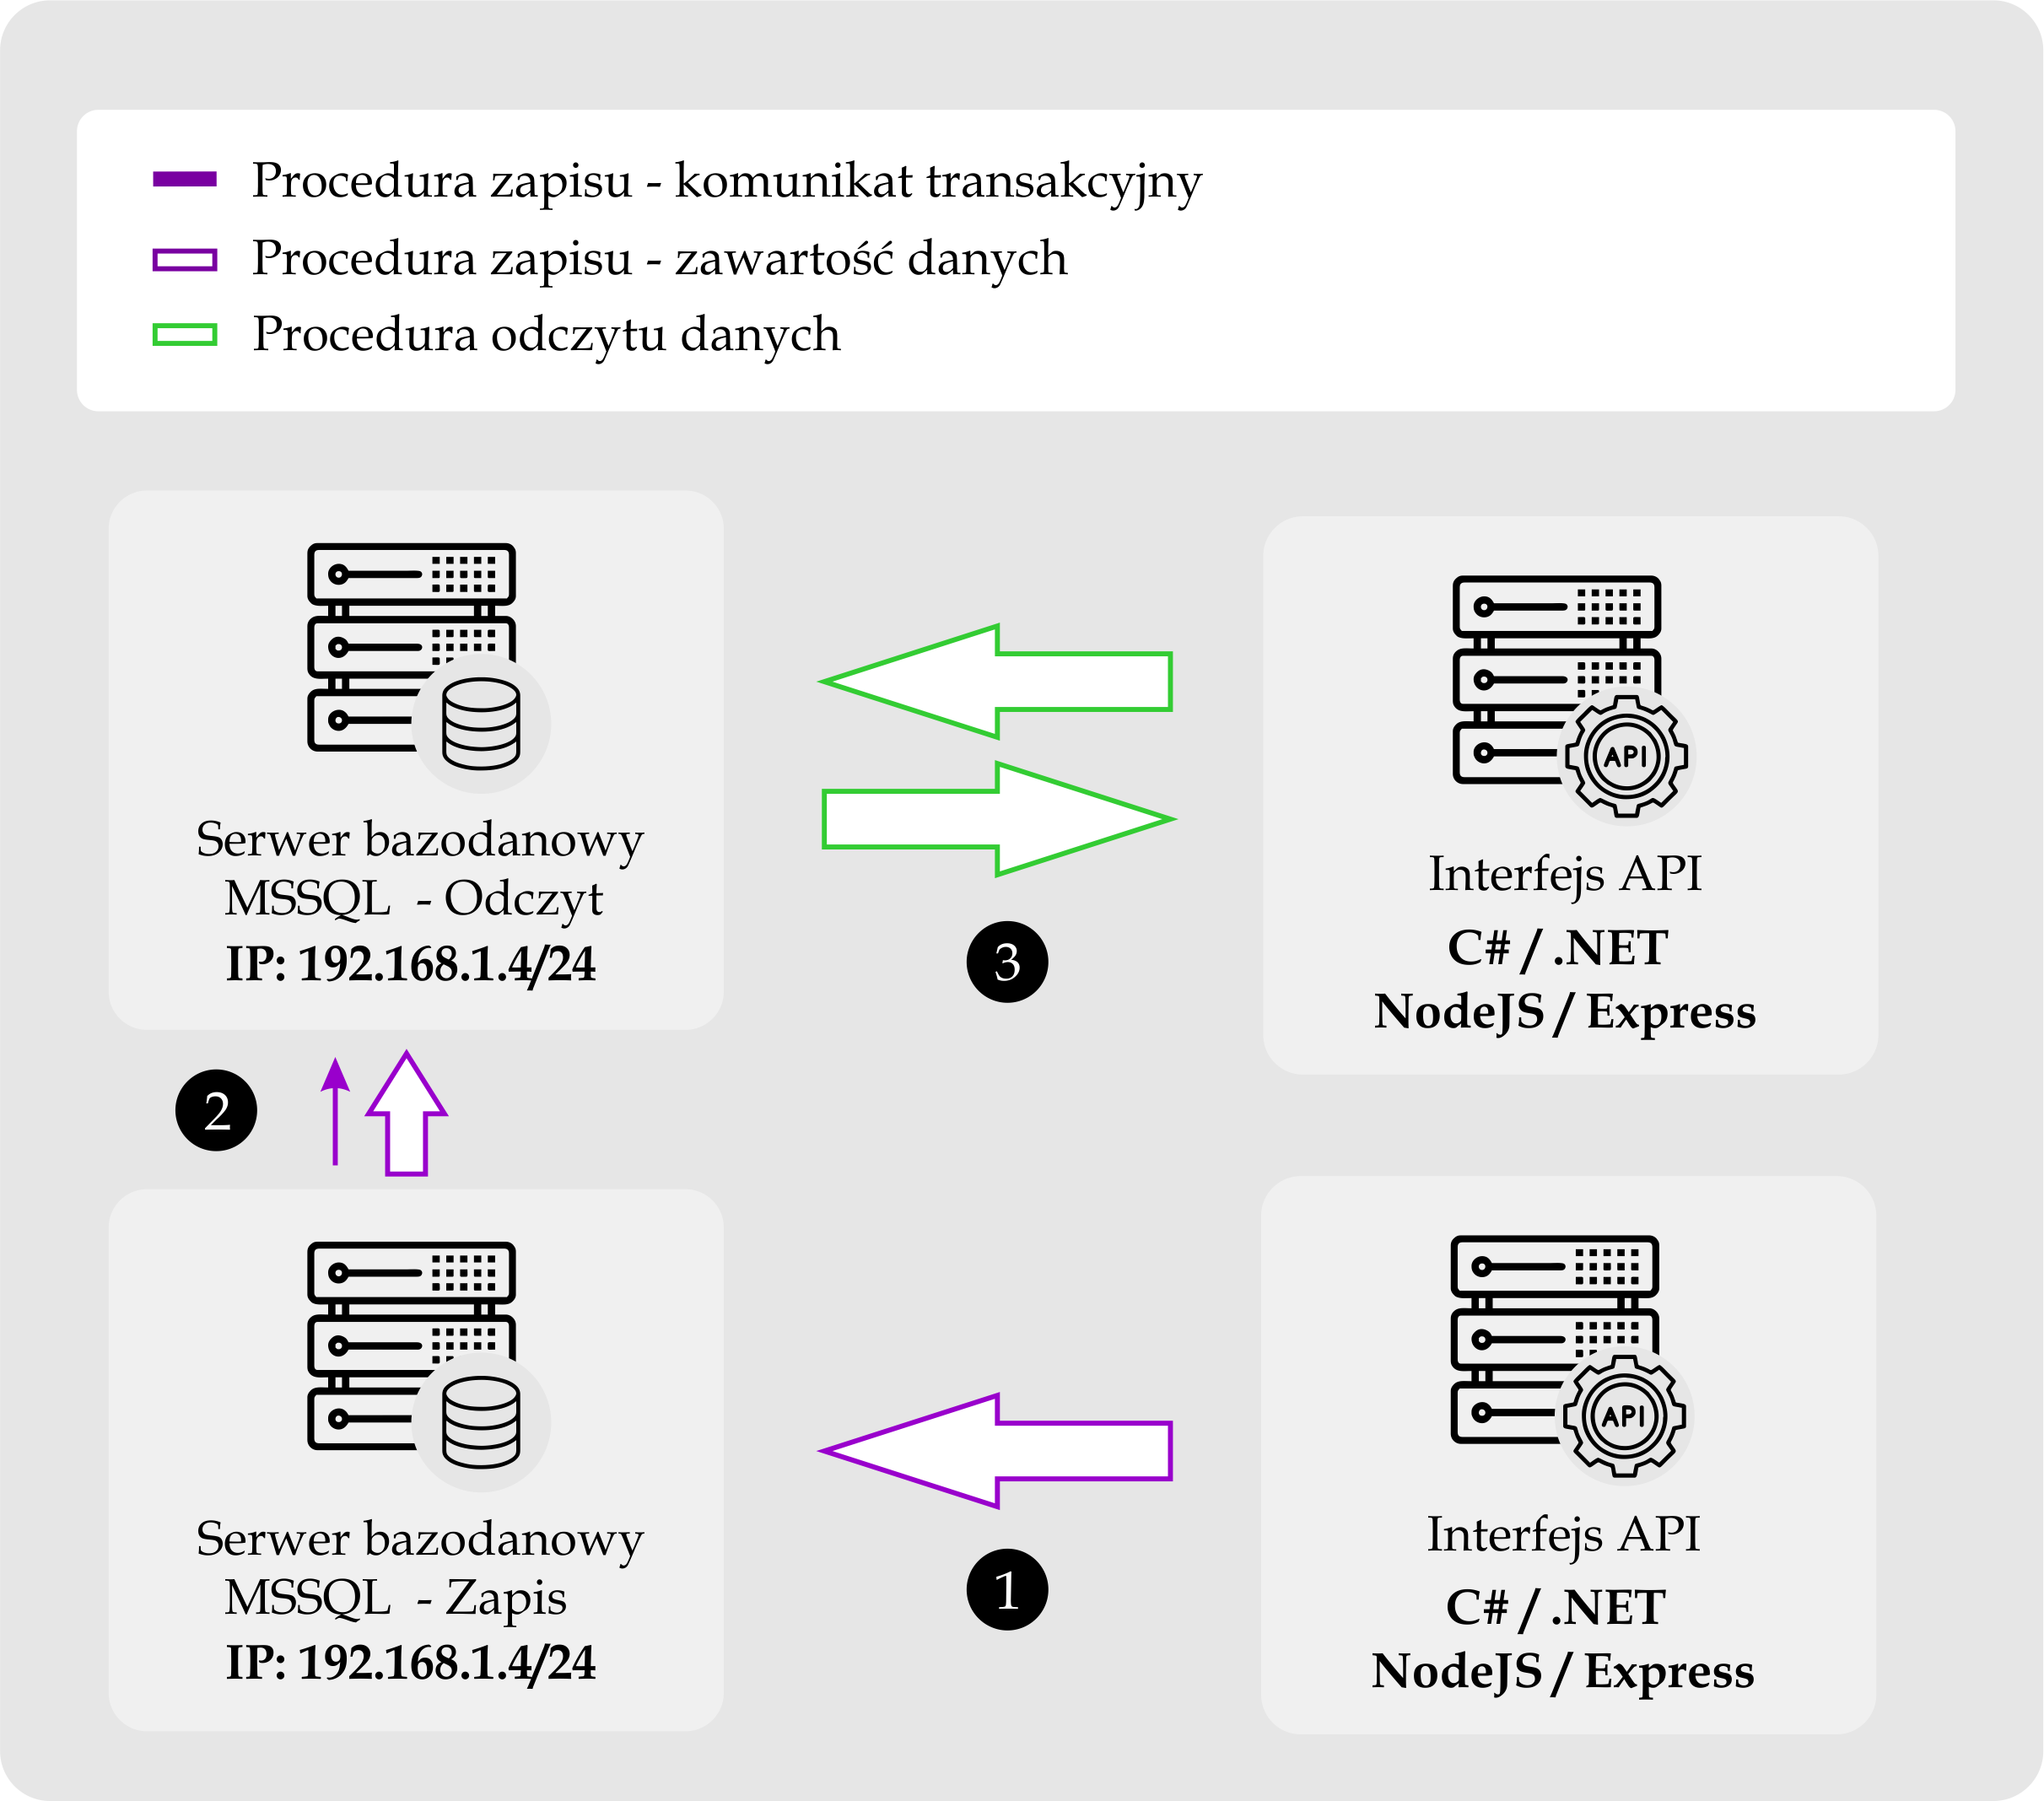
\includegraphics[width=\linewidth]{rys04/jak_dziala_transakcja.png}
    \caption{Schemat wykonywania procedur zapisu oraz odczytu z wykorzystaniem replikacji transakcyjnej}
    \label{fig:jak-dziala-replikacja}
\end{figure}

Zastosowanie omówionego mechanizmu pozwoliło na dokonanie implementacji interfejsów programowania aplikacji, które mogą zarówno uwzględniać dwa odrębne, zoptymalizowane względem typu operacji modele danych, jak i manipulować danymi bez ryzyka wystąpienia nadmiernego opóźnienia wynikającego z konieczności wykonania synchronizacji na poziomie API.   

Podstawową intencją dokonania separacji środowisk zapisu i odczytu, a także wykorzystania wzorca projektowego podziału odpowiedzialności jest możliwość wdrożenia optymalizacji modelu odczytu danych. Optymalizacje te, zarówno dotyczące struktur bazodanowych, jak i rozwiązań programistycznych, mają na celu przyspieszenie procedury odwoływania się, pozyskiwania oraz zwracania danych bezpośrednio do aplikacji klienckiej.  

Zależnie od wykorzystywanej technologii, możliwe było wprowadzenie różnych rozwiązań optymalizacyjnych dotyczących zarówno struktur bazodanowych, jak i generowania zapytań w kierunku bazy danych.

W ramach interfejsu programowania aplikacji uruchamianego w środowisku .NET/C\# wprowadzono następujące usprawnienia wydajnościowe:
\begin{itemize}
    \item Kompilowane kwerendy \textit{(ang. Compiled Queries)} - zapytania o dane linq, wykorzystywane przez mapper entity framework core stanowią intuicyjny i prosty w budowie interfejs komunikacji z systemem bazodanowym. Programista, w nieskomplikowany sposób może zbudować zaawansowaną kwerendę pozyskującą dane, odwołującą się jednocześnie do wielu struktur bazodanowych. Rozwiązanie to jednak, wymaga zbudowania przez bibliotekę entity framework core drzewa składniowego reprezentującego kwerendę i pozwalającego na jej przekształcenie do kodu języka bazy danych. Proces ten, wraz ze zwiększeniem się poziomu skomplikowania zapytania może trwać znacząco dłużej i wpływać negatywnie na wydajność aplikacji. Dlatego też, zastosowano się na wykorzystanie podejścia kompilowanych kwerend, które pozwala na zbudowanie drzew składniowych dla zapytań jednokrotnie po uruchomieniu api, a następnie szybsze generowanie kodu języka bazy danych.
    \item Pula kontekstów bazodanowych \textit{(ang. DbContext Pool)} - dla standardowej konfiguracji interfejsów API w ramach platformy .NET, instancja klasy kontekstu bazodanowego inicjalizowana każdorazowo dla pojedynczego żądania wysyłanego w kierunku API. Rozwiązanie to jest akceptowalne przy standardowym natężeniu otrzymywanych żądań ze względu na niewielki rozmiar instancji klasy, a także szybki czas jej ustanowienia. W przypadku zwiększonego natężenia ruchu sieciowego w kierunku API, wydajność może zostać z tego powodu obniżona. W celu zapobiegania spadku wydajności zastosowano mechanizm puli obiektów kontekstu bazodanowego. Mechanizm ten pozwala na utrzymywanie wielu obiektów konktekstu przez cały czas działania API i czasowe przydzielanie tych obiektów do obsługi nadchodzących żądań.
    \item Leniwe ładowanie \textit{(ang. Lazy loading)} - domyślnym zachowaniem obiektu kontekstu bazodanowego jest wykonanie kwerendy tuż po jej deklaracji, a także pozyskanie wszelkich obiektów nawigacyjnych, które zostały w niej wymienione. Zachowanie to, powoduje pozyskanie określonych fragmentów danych, które zostaną wykorzystane dopiero w dalszej części przetwarzania programu. Mechanizm leniwego ładowania pozwala na pozyskiwanie danych dopiero wtedy, gdy instrukcje kodu źródłowego wskazują na konieczność ich wykorzystania.
    \item Rozdzielone zapytania \textit{(ang. Split Queries)} - kod języka bazy danych, wygenerowany poprzez przetworzenie drzewa składniowego zapytania linq przez entity framework core, domyślnie uwzględnia pozyskiwanie encji zależnych (tj. encji identyfikowanych kluczem obcym) poprzez dokonanie lewostronnego iloczynu kartezjańskiego. Dzięki temu, niezależnie od tego, ile encji zależnych programista będzie chciał uzyskać, operacja pozyskiwania danych sprowadzona zostanie do pojedynczego zapytania. Wiąże się to jednak z możliwością uzyskania bardzo dużej liczby zduplikowanych danych. Dane te, są programowo filtrowane przez maper obiektowo-relacyjny przed zwróceniem ich do kodu programu. Aby uniknąć konieczności redukcji zduplikowanych danych, przy założeniu wykonywania kwerend dołączających wiele encji zależnych wykorzystany został mechanizm rozdzielonych zapytań, który przekształca pojedyncze zapytanie z wielokrotnym lewostronnym iloczynem w serię kilku osobnych zapytań.
    \item Pula połączeń bazodanowych \textit{(ang. Database Connections Pool)} - zdefiniowanie parametru obsługi wielu równolegle działających połączeń z serwerem bazodanowym. 
\end{itemize}

Ponadto, wprowadzono wiele mniej znaczących usprawnień wydajnościowych, takich jak przekazywanie parametrów do zapytań linq zamiast stosowania stałych dosłownych, czy też redukcja wykorzystania zewnętrznych metod wewnątrz funkcji anonimowych zapytania. 

W ramach interfejsu programowania aplikacji uruchamianego w środowisku NodeJS/Express wprowadzono następujące usprawnienia wydajnościowe:
\begin{itemize}
    \item Wykorzystanie obiektu include do dołączania encji zależnych w sposób kontrolowany przez mapper obiektowo-relacyjny prisma, tak aby zredukować możliwość wystąpienia problemu n+1 zapytań.
    \item Zdefiniowanie pojedynczej, globalnej instancji klienta mappera obiektowo-relacyjnego \textit{PrismaClient}, w celu redukcji konieczności każdorazowego dokonywania operacji zajęcia i zwolnienia pamięci, a także czasu potrzebnego na nawiązanie połączenia pomiędzy klientem a instancją systemu bazodanowego.
    \item Pula połączeń bazodanowych - zdefiniowanie parametru obsługi wielu równolegle działających połączeń z serwerem bazodanowym. 
\end{itemize}

Co więcej, wprowadzono również następujące optymalizacje wydajności ściśle dotyczące struktur bazodanowych:
\begin{itemize}
    \item Zdefiniowanie indeksów oraz określenie pól jako unikalne w celu przyspieszenia procesu odwoływania się do danych, a także ich filtracji oraz sortowania
    \item Ograniczenie przedziałów liczbowych dla pól numerycznych oraz maksymalnych długości dla ciągów tekstowych
    \item Przekształcenie określonych pól ciągów tekstowych z typu \textit{NVARCHAR} wykorzystującego do kodowania pojedynczego znaku 2 bajty (kodowanie UTF16), do typu \textit{VARCHAR} wykorzystującego do kodowania pojedynczego znaku jeden bajt.
\end{itemize}
\section{Konfiguracja generycznych oraz dedykowanych platform chmurowych}
W kontekście przeprowadzanych ewaluacji skonfigurowano trzy platformy chmurowe, w ramach których uruchomiono badane interfejsy programowania aplikacji. Wykorzystanie odmiennych platform chmurowych jako środowisk wdrożeniowych dla interfejsów API ma na celu dokonanie obserwacji zmiany wydajności działania systemów internetowych względem poziomu przystosowania usługi wdrożeniowej w odniesieniu do konkretnego interfejsu programowania aplikacji. Oznacza to, że ewaluowane zostały zarówno rozwiązania o wysokim stopniu ogólności (tj. dostarczające możliwości pełnego zarządzania systemem operacyjnym serwera, na którym wdrożone zostały aplikacje), jak i te, które bezpośrednio powiązane są z określoną technologią implementacyjną.

W ramach pierwszej z omawianych platform chmurowych, wykorzystano usługę typu \textit{Infrastructure as a Service} w postaci wirtualnego serwera prywatnego udostępnionego przez dostawcę usług chmurowych \textit{DigitalOcean}. Serwer ten, posiadał 25GB pamięci dyskowej, 16GB pamięci operacyjnej o dostępie swobodnym, a także ośmiordzeniową centralną jednostkę przetwarzania o architekturze 64-bitowej. Na omawianym serwerze zainstalowano dystrybucję systemu operacyjnego Linux o nazwie \textit{Ubuntu Server} w wersji 22.04 LTS.

Niezależnie od technologii wdrażanego interfejsu programowania aplikacji, zdecydowano się na wykorzystanie tego samego serwera usługi WWW, którym w tym przypadku było oprogramowanie \textit{Apache2}. Usługa ta, pełniła rolę odwróconego serwera pośredniczącego \textit{(ang. Reverse-proxy)}, pomiędzy serwerem interfejsu API a zlokalizowanymi na zewnątrz sieci urządzeniami klienckimi. Serwerem interfejsu API napisanego w języku C\# było oprogramowanie \textit{Kestrel}, natomiast w przypadku NodeJS API, usługą wykorzystywaną do hostowania aplikacji w środowisku lokalnym był framework \textit{ExpressJS}. Oba, spośród wymienionych serwerów aplikacji uruchomione były w obrębie systemu operacyjnego w postaci programów typu demon działających w tle. Oprogramowanie poszczególnych interfejsów programowania aplikacji uruchomione było tylko na czas przeprowadzania ewaluacji i nigdy nie funkcjonowało w sposób równoległy.

Drugi z zastosowanych mechanizmów wdrożeniowych to rozwiązanie typu \textit{Platform as as Service} udostępniane przez dostawcę usług chmurowych \textit{Microsoft Azure}. W tym przypadku, programista zarządzać może uruchomionymi usługami, określać konfigurację każdej z nich, natomiast nie posiada on dostępu do warstw uruchamiania programów, czy też administrowania systemem operacyjnym. Aby zapobiec niereprezentatywności wyników badań przeprowadzanych w obrębie przedstawianego środowiska chmurowego, zdecydowano się na skorzystanie z opcji dynamicznego przydziału zasobów sprzętowych do skonfigurowanych usług, z zastrzeżeniem maksymalnych wartości pojemności dyskowej do 25GB, pamięci RAM do 16GB, a także liczby wykorzystywanych rdzeni centralnej jednostki przetwarzania do ośmiu. Na omawianej platformie uruchomiono usługę interfejsu programowania aplikacji napisanego w języku C\# z wykorzystaniem platformy .NET, a także system bazodanowy Microsoft SQL Server.

Odnosząc się do ostatniej spośród eksploatowanych platform chmurowych, zastosowano rozwiązanie typu \textit{Platform as a Service} dostawcy usług \textit{Heroku}. Rozwiązanie to, jest rekomendowanym sposobem wdrożenia aplikacji internetowych opartych o środowisko NodeJS. Analogicznie do platformy udostępnianej przez dostawcę DigitalOcean, w przypadku usługi Heroku istnieje możliwość doboru komponentów sprzętowych dostępnych w ramach fizycznej maszyny hostującej. W związku z tym faktem, a także w celu zapobiegania uprzywilejowaniu któregokolwiek z rozwiązań w kontekście przeprowadzanych badań, zastosowano te same wartości pojemności dyskowej, pojemności pamięci operacyjnej, a także liczby rdzeni procesora. Dostęp do systemu operacyjnego urządzenia serwerowego, zgodnie z typem przedstawianej usługi, nie jest przyznany użytkownikowi. Na omawianej platformie uruchomiono usługę interfejsu programowania aplikacji napisanego w języku JavaScript z wykorzystaniem platformy NodeJS/Express, a także nierelacyjny system bazodanowy MongoDB.
\section{Konfiguracja narzędzia do realizacji badań}


